\documentclass[a4paper, french, 12pt]{article}  % DŽclare la classe du document.
% Il existe 5 classes sous LaTeX : article, book, report, letter et slides 
% Les options de classe sont entre crochets et permettent de faire des choix d'ordre gŽnŽral :
% - dŽfinir la taille de base des caractres avec 10pt, 11pt, 12pt, les commandes d'agrandissement 
% ou de rŽduction de la tailles des caractres ( \small \large ) se feront alors par rapport ˆ cette base
% - dŽfinir la taille du papier:  a4paper,  a5paper, b5paper, executivepaper, legalpaper ou letterpaper
% Utiliser a4paper ds que la papier utilisŽ est de ce format c'est ˆ dire ... tout le temps ;-)
% - utiliser des options de mise en page : 
%       ->   landscape passe en mode paysage pour l'ensemble du doccument
%       ->   onecolumn  option par dŽfaut, le texte sera sur une seule colonne 
%       ->   twocolumn   pour un doccument sur deux colonnes, des rŽglages sont possibles (cf doc & net)
%       ->   oneside toutes les pages seront traitŽs identiquement, par dŽfaut avec la classe article
%       ->   twoside  mise en page diffŽrentes pour les pages pairs et impairs par dŽfaut avec book
%       ->   openright et openany  pour gŽrer le commencement des chapitres dans la classe book
%       ->   titlepage et notitlepage indique si une nouvelle page doit tre commencŽe aprs le titre du document.

% \usepackage permet de dŽclarer un module qui sera pris en compte dans la suite. 
% Les modules permettent d'Žtendre les fonctionnalitŽ de LaTeX

%%%%Caracteres reserves%%%%%%%%%%%
%Pour les obtenir on les fait précéder d'un \
% { s'obtient avec \{
% } s'obtient avec \}
% % s'obtient avec \% 
% $ s'obtient avec \$
% & s'obtient avec \&
% # s'obtient avec \#
% _ s'obtient avec \_
% ^ s'obtient avec \^{}
% \ s'obtient avec \textbackslash{} car \\ est une commande
%Les caractères [ et ] ne sont pas réservés et s'obtiennent directement
%\[ et \] delimitent une environnement mathematique
%%%%%%%%%%%%%%%%%%%%%%%%%%%%%%%%%%%%%%%%%%%


%%%%%Polices%%%
%La police employee par defaut par Latex s'appelle Computer Modern

%%%Changement de style de police%%

%Police par defaut {\normalfont ...} c'est une bascule

%Trois familles 
%Romaine par defaut
%sans serif \textsf{..} ou {\sffamily ....}
%typewriter \texttt{..} ou {\ttfamily ....}

%Quatre formes
%droite par defaut
%italique \textit{..} ou {\itshape ....}
%penchee \textsl{..} ou {\slshape ....}
%petites capitales  \textsc{..} ou {\scshape ....}

%Deux series
%normale par defaut
%grasse \textbf{..} ou {\bfseries ....}


%%Taille%%
%Toutes les commandes suivantes sont des bascules a utiliser entre accolades
%{\tiny petit mot}
%Dans l'ordre croissant
%\tiny
%\scriptsize
%\footnotesize
%\small
%\normalsize
%\large
%\Large
%\LARGE
%\huge
%\Huge

%%%%%%%%%%%%%%%%%%%%%%%%%

%%%%%Justification%%%%%
%Alignement a droite
%\begin{flushright}
%{\raggedleft texte \par} ne pas oublier \par
%\leftline{texte}
%\filleft pour formater un titre 

%Alignement a gauche
%\begin{flushleft}
%{\raggedright texte \par} ne pas oublier \par
%\rightline{texte}
%\filright pour formater un titre 


%Centrage
%\begin{center}
%{\centering texte \par} ne pas oublier \par
%\centerline{texte}
%\filcenter pour formater un titre 
%%%%%%%%%%%%%%%%%%%%%%%%%%%%%%%%%%%%%%%%%%%

%%%%%%Espaces%%%%%%%%%%%%%%%%%%%%%


%%Espaces verticaux%%%
%\vskip 2cm  (argument eventuellement negatif), l'espace est ignore s'il coincide avec un saut de page
%\vspace*{2cm} (argument eventuellement negatif), l'espace n'est pas ignore s'il coincide avec un saut de page
%\vspace{2cm} est synonyme de \vskip 2cm 

%%Espaces horizontaux%%%%

%\hskip equivalent a \vskip
%\hspace{?} et \hspace*{?}
%Le cadratin est un espace horizontal egal a la taille de la police utilisee
%\thinspace espace d'un sixieme de cadratin
%\enskip pour un demi-cadratin
%\quad pour un cdratin
%\qquad pour deux cadratins

%%%%%%%%%%%%%%%%%%%%%%%%%%%%%%%%%%%%

%Le moteur eTeX est aujourd'hui utilisé par toutes les distributions (MikTeX, TeXlive) à la place de l'ancien TeX (en fait, c'est plutôt PDFTeX, le successeur de eTeX, qui est utilisé ; contrairement à ce que son nom indique, il peut produire du dvi). Le fait d'utiliser le moteur eTeX au lieu de TeX donne accès à des choses en plus (par exemple à \middle pour aller avec \left et \right, mais aussi à des commandes bien pratiques comme \numexpr, \dimexpr, \detokenize, etc. ainsi qu'à des ressources supplémentaires, comme plus de compteurs disponibles).

%Lorsqu'on utilise le moteur eTeX, certaines de ces fonctionnalités sont automatiquement accessibles (c'est le cas de \middle, \numexpr, etc.), mais pas d'autres (c'est le cas des compteurs supplémentaires). Pour activer ces fonctionnalités manquantes, on peut charger le package etex.sty. Ainsi, l'utilisation d'etex.sty est une solution courante au problème d'avoir trop de compteurs définis (c'est le cas si on charge ensemble trop de packages du type tikz, pstricks, xymatrix, ...)

\usepackage{etex}

%%%%%%%%%%%%Encodage du fichier source %%%%%%%%%%%
\usepackage[T1]{fontenc}
\usepackage[utf8]{inputenc}


%%%%%%%%%%%%%%%Francisation%%%%%%%%%%%%%%
\usepackage[french]{babel}
\frenchbsetup{StandardLists=true}
%%%%%%%%%%%%%%%%%%%%%%%%%%%%%%%%%%%%%%%%%

%%%%%%%%%%%%Mise en page, Reglages genrraux%%%%%%%

%\title{il n'existe pas de plus grand nombre premier}
%\author[Euclide \thanks{Merci Aristote}}
%\date{12 juin $-260$}  Par défaut Latex insère la date du jour
%puis écrire après \begin{document} la commande \maketitle


\usepackage[a4paper,headheight=35 pt, headsep=15pt,top=20 pt,hmargin=1 cm,bottom=20 pt,includeheadfoot]{geometry}
%\usepackage[a4paper,hmargin=1 cm,bottom=2cm,top=2cm,headheight=15pt]{geometry}      
%top est la marge supérieure entre le haut de body et le bord supérieur de la feuille
% \usepackage[left= 4cm,right = 3cm,top= 2cm, bottom=2cm]{geometry} pour le réglage des marges 
% \usepackage[top= 17mm,textheight=23cm,heightrounded,left=25mm,textwidth=16cm] {geometry} pour fixer la hauteur,  la largeur  du texte. heightrounded, autorise le package à arrondir la hauteur textheight à un nombre entier de lignes pour éviter des problèmes de remplissage vertical underfull vbox 


\usepackage{setspace}  % pour le réglage de l'interligne
%Bascule \doublespacing  ou environnement {doublespace}
%Bascule \onehalfspacing  ou environnement {onehalfspace}
%Bascule \singlespacing  ou environnement {singlespace}
% ou encore \renewcommand{\baselinestretch}{n} ou encore l'environnement spacing{n}

%%Package fullpage
%\usepackage[cm]{fullpage}
%where possible options for fullpage are
%in (default) sets the margins to one inch;
%cm sets the margins to 1.5 cm (one centimeter is really too
%little);
%plain (default) selects the plain page style, i.e., with no head-
%ers but only a footer;
%empty for neither headers nor footers;
%headings for both header and footers;
%myheadings also for both headers and footers.
%For the last 4 options, the corresponding \pagestyle declaration is exe-
%cuted, so that it is not necessary to give it again.


%%Pour la numerotation des bas de pages avec le compteur lastpage%%%
\usepackage{lastpage}

%%%%Pour afficher certaines pages au format paysage%%
\usepackage{lscape}
%\begin{landscape}

%%%Plusieurs colonnes
\usepackage{multicol}
%\begin{multicols}[titre]{nb colonnes}
\setlength{\columnseprule}{0.25pt}


%%%%%Références, Notes de bas de pages ou de marges%%%%%%%%%

%%Pour placer une note de bas de page : commande \footnote{}
%Pour placer une note dans la marge : \marginpar{}
%Pour plcaer une note dans un tableau : appel de note avec \footnotemark{} puis le texte après le tableau avec \footnotetext{texte}

%Etiquette  avec \label{nom} puis référence à l'étiquette (numéro de section le plus proche ) avec \ref{nom} ou à lap age avec \pageref{nom}
\usepackage{varioref}
%Introduit  les commandes \vref{} et \vpageref{} qui améloirent l'affichage ainsi que la commande \vpagerefrange{label1}{label2} pour faire référence à tout un bloc de pages entre deux étiquettes
\usepackage{nameref}


%%%%Présentation des titres de section%%%

%\usepackage[clearempty]{titlesec} problème avec PDFLatex ?

%Pour changer la police des titres de sectionnement, un exemple :
%\titleformat*{\section}{\sffamily}

%Pour modifier la police mais aussi la présentation :
%\titleformat{commande}[shape]{format}{label}{sep}{before}{after}
% commande est la commande de sectionnement comme \section
%shape peut etre hang (défaut),frame (encadre), display( paragraphe séparé), block (paragraphe), runin (dans le texte, wrap (comme wrapfigure), leftmargin ou rightmargin
%format est le formatage du titre complet (numéros inclus)éventuellemnt précédé de commandes à inclure avant le titre
% Ces commandes peuvent etre \titleline[r,c ou l]{texte} ou \titlerule[epaisseur] ou \titlerule*[epaisseur]{texte}
%label est la présentation du numero
%sep est l'espace entre le numero et le titre
%before est le code à exécuter avant le titre de section (numero exclu)
%after est le code à exécuter après (vide en général)

%Pour gérer l'espacement
%\titlespacing{commande}{left}{beforesep}{aftersep}[right]
%left est la marge à gauche, beforesep l'espace vertical avant etc ..


%Exemple de présentation de titre encadé :
%\titleformat{\section}[frame]{\titleline[r]{\rule{2in }{2pt}} \normalfont}{\filright\small\ SECTION \thesection\hfill}{7pt}{\LARGE \bfseries\filcenter}{}
%\section{un titre de section encadre}


%%%%%%%%%%%%%%%%%%%%%%%%%%%%%%%%%%%%%%%%%%%% 

%%%%%%%Réglages de la table des matières%%%%
\usepackage{tocvsec2}
%Définir la progondeur : \setcounter{tocdepth}{1}  :
%1 correspond aux chapitres; 2 aux sections etc ...
%Rédéfinir le nom par défaut  :
%\renewcommand{\contentsname}{Liste des chapitres}
%Modifier une entrée :
%\Chapter[titre court]{titre long}
%Ajouter une entrée :
%\addcontentsline{toc}{section}{Nom de la section qu'on veut ajouter}
%Pour exclure une entrée 
%Utiliser une commande étoilée comme \section*
%Pour ajouter  ce qu'on veut dans la table des matières comme des indications de mise n page :
%\addtocontents{toc}{\protect \pagebreak}


%%%%%%%%%%%% Packages pour le texte %%%%%%%%%%%%
\usepackage{lmodern}       %Joli fonte

\usepackage{pifont,fourier}
\usepackage[normalem]{ulem}
%\uline{} pour  un soulignement simple
%Commmandes \uuline{} pour un soulignement double
%\uwave{} pour un soulignement  avec des vagues
% \sout{} pour barrer et \xout{} pour hachurer
\usepackage{cancel} %Commande \cancel{} pour barrer en oblique
%\usepackage{soul}    %souligner
%\usepackage{lettrine} %Pour commencer un paragraphe avec une lettrine
%Package incompatible avec tabvar.tex
%\lettrine{S}{i vous souhaitez}
%\renewcommand{\LettrineFontHook}{\itshape}
%\renewcommand{\LettrineTextFont}{\sffamily}

%%%Pour des jolis boites%%%
\usepackage{fancybox}  
%Commandes \box{} \ovalbox{} \shadowbox{}
%\cornersize{}2 réglage de l'arrondi
% Dimension à régler avec \setlength{}  : \fboxsep \fboxrule  

%%% Pour faire tourner le texte %%%
\usepackage{rotating}  %\begin{turn}{-60} tourné \end{turn} pour tourner un paragraphe
						%pour tourner un texte, commande \rotatebox[origin=c]{angle}{texte}
						
%%Divers%%%%
\usepackage{eurosym}  %pour le symbole de l'euro

\usepackage{url} %pour la gestion des adresses web avec la commande \url{}

%%%%%%%%%%%

%%%%%%%%%%%%%%%Ecriture d'algorithmes Insertion de code source %%%%%%%%%%%

%%%%%Package verbatim%%%%

\usepackage{verbatim} 
%LE package verbatim améliore la présentation des verbatim
% Il  fournit un environnement {comment} pour insérerer des commentaires
%dans le fichier source sans faire précéder toutes les lignes de %

\usepackage{alltt, moreverb} 
%L'environnement verbatimboxed permet d'encadrer un texte en verbatim
% De plus les caractères spéciaux \ et { ne sont pas désactivés (mais #, $ et % le sont)
% et on peut saisir des formules mathématiques avec \( .. \) ou \[ ... \]

%%Pour améliorer envore la présentation des verbatim%%%%
\usepackage{fancyvrb}


%%Couleur
\usepackage[table]{xcolor}
% options : rgb,cmyk,gray,hsb,html pour transformer automatiquement toutes les couleurs du docuement dans le mode choisi
%\definecolor{mauve}{rgb}{0.7,0,0.43}
%\color{couleur} bascule
%\textcolor{couleur}{texte}
%\pagecolor{couleur}
%\colorbox{couleur}
%\fcolorbox{couleur}




%%%%%%%%%% Nouvelles couleurs
\definecolor{rouge}{rgb}{1,0,0}
\definecolor{bleu}{rgb}{0,0,1}
\definecolor{orange}{rgb}{1.00,0.50,0.00}
\definecolor{vert}{rgb}{0,0.50,0.00}
\definecolor{marron}{rgb}{0.49,0.16,0.06}
\definecolor{mauve}{rgb}{0.42,0.24,0.77}
\definecolor{rpastel}{rgb}{1.00,0.77,0.77}
\definecolor{bpastel}{rgb}{0.70,0.86,0.93}
\definecolor{grisclair}{gray}{0.85}
\definecolor{gristclair}{gray}{0.95}
\definecolor{grisfonce}{gray}{0.4}

%%%%%%%%%%%%%%%%%%¨Puce, Listess%%%%%%%%%%%%%%
\usepackage{enumerate}
\usepackage{enumitem}
%Pour changer la puce de liste dans tout le document :
%AtBeginDocument{\renewcommand{\labelitemi}{\textbullet}}
%%%%%%%%Réglages spécifiques au document%%%%%%%%%

%\setenumerate[1]{label=\textbf{Q\arabic*)}}


%%%%%%%%%%%%Graphiques et Dessins%%%%%%%%%%%%%%

\usepackage{graphicx}		
%\rotatebox[origin=x0x1]{angle}{texte} avec xox1 parmi t (top) l (left) r (right) B (ligne de base) et b (bottomm)
%\resizebox{largeur}{hauteur}{texte} pour faire rentrer u nelement encombrant dans une boite					


\usepackage{epic,eepic}   %Capacités graphiques étendues
%\begin{picture}(0,0) permet d'insérer n'importe quoi, n'importe où sans prendre de place (utilie pour annoter une figure en eps)
%Une autre technique est \makebox[0cm][alignement]{texte}
%Exemple:
%\includegraphics[scale=1]{singe.eps}
%\begin{picture}(0,0)
%\put(-27,10){$\sqrt[3]{8}$}
%\end{picture}



%%%%%%%%%%PSTricks%%%%%%%%%%%%

\usepackage{pstricks,pst-plot,pst-text,pst-tree,pst-eps,pst-fill,pst-node,pst-math,pstricks-add,pst-xkey,pst-eucl}


%%%%%%%Tikz%%%%%%%%%%%%%%%
\usepackage{pgf,tikz,tkz-tab}
% Pour les tableaux de signes ou de variations avec tkz-tab voir https://zestedesavoir.com/tutoriels/439/des-tableaux-de-variations-et-de-signes-avec-latex/#1-13389_tikz-un-package-qui-en-a-dans-le-ventre
\usetikzlibrary{arrows}
\usetikzlibrary{shapes.geometric}
\usetikzlibrary{shapes.geometric}
\usetikzlibrary{petri}
\usetikzlibrary{decorations}
\usetikzlibrary{arrows}
\usetikzlibrary{math}
 %Variables must be declared in a tikzmath environment but
       % can be used outside
%       \tikzmath{int \n; \n = 508; \x1 = 1; \y1 =1; 
%                   %computations are also possible
%                    \x2 = \x1 + 1; \y2 =\y1 +3; } 


%%%%%%%%%%%%%%%%%%%%%%%%%%%%%%%%%%%%%%%%
%%%%%%%%%%%Commandes Tikz Perso%%%%%%%%%%%%%%%

% Définition des nouvelles options xmin, xmax, ymin, ymax
% Valeurs par défaut : -3, 3, -3, 3
\tikzset{
xmin/.store in=\xmin, xmin/.default=-3, xmin=-3,
xmax/.store in=\xmax, xmax/.default=3, xmax=3,
ymin/.store in=\ymin, ymin/.default=-3, ymin=-3,
ymax/.store in=\ymax, ymax/.default=3, ymax=3,
}
% Commande qui trace la grille entre (xmin,ymin) et (xmax,ymax)
\newcommand {\grille}[2]
{\draw[help lines,black, thick] (\xmin,\ymin) grid[xstep=#1, ystep=#2] (\xmax,\ymax);}
% Commande \axes
\newcommand {\axes} {
\draw[->,very thick] (\xmin,0) -- (\xmax,0);
\draw[->,very thick] (0,\ymin) -- (0,\ymax);
\draw (0.95*\xmax, 0) node[above] {$x$};
\draw (0, 0.95*\ymax) node[left] {$y$};
}
% Commande qui limite l?affichage à (xmin,ymin) et (xmax,ymax)
\newcommand {\fenetre}
{\clip (\xmin,\ymin) rectangle (\xmax,\ymax);}

%Exemple d'utilisation

%\begin{center}
%\begin{tikzpicture} [xmin=-2,xmax=2,ymin=0,ymax=5]
%\grille{1} \axes \fenetre
%\draw plot[smooth] (\x,\x^2);
%\end{tikzpicture}
%\end{center}

%style pour la perspective cavalière française
%voir Tikz pour l'impatient page 68
\tikzset{math3d/.style=
{x= {(-0.353cm,-0.353cm)}, z={(0cm,1cm)},y={(1cm,0cm)}}}

%%%%%%%Symbole pour code calculatrice%%%%%%

%Flèche remplie pour défilement de menu

\newcommand{\flechefillright}{
\begin{tikzpicture}[scale=0.15] \fill (0,0)--(2,1)--(0,2)--cycle;
\end{tikzpicture}}

%%%%%%%%%%%%%Symboles pour calculatrice Casio%%%%
\newcommand{\execasio}{\Pisymbol{psy}{191}} %Retour chariot
\newcommand{\dispcasio}{\begin{pspicture}(.1,.1)\pspolygon*(.1,0)(.1,.1)\end{pspicture}} %Triangle « Disp »
\newcommand{\dispcasiotikz}{\begin{tikzpicture}[scale=0.2]
\fill (0,0) -- (1,0) -- (1,1) -- cycle;
\end{tikzpicture}} %Triangle « Disp »
%

%Fleche entre deux lignes, d'apres 'un bon petit' : http://forum.mathematex.net/latex-f6/fleches-entre-deux-lignes-pour-resolution-d-equation-t10283.html#p99817
\newcommand\addnode[1]{\Rnode{#1}{}}
\newcommand\linknode[3]{\ncbar[angleA=0,angleB=0,nodesep=1ex,arm=10ex,offset=-2pt]{->}{#1}{#2}\Aput{\vphantom{x}#3}}


%%Commande pour touche de calculatrice

\newcommand\tc[1]{%
{
\begin{tikzpicture}
\node[draw,rectangle,rounded corners=3pt] (P) at (0,0){#1};
\end{tikzpicture}
}
}

%%%%%%%%%%%%%%%%%%%%%%%%%%%%%%%%%%%%%%%%
%%%%%%%%%%%Fin Commandes Tikz%%%%%%%%%%%%%%%


%%%%%%%%%%%%Specifiques%%%%%%%%%%%
\usepackage{wrapfig}
%pour insérer une figure à droite ou à gauche d'un texte
%\begin{wrapfigure}[nb lignes]{placement l,r,c,i(inside),o(outside)}[overhang]{width}
%ce package fonctionne mal à proximité des listes
%%%%%%%%%%%%%%%%%%%%%%%%%%%%%%%%%%%%%

%%%%%Environnements et symboles spéciaux pour faire joli%%%%%%

%%%Bclogo, pour des environnements + jolis avec insertion de logo%%%%
%Dépendances de  bclogo
\usepackage{xkeyval}  
\usepackage{etoolbox}
\usepackage{ifpdf}
\usepackage[framemethod=tikz]{mdframed}
\usepackage[tikz]{bclogo}

%\newcommand\bcpython{
\includegraphics[width=17pt]{/home/fjunier/Maths/python-logo.eps}}
\newcommand\bcpython{
\includegraphics[width=17pt]{python-logo.png}}
%\newcommand\bcpython{
\includegraphics[width=17pt]{/home/frederic/Maths/python-logo.png}}

%% Framed
\usepackage{framed}  %Le package « framed» Crée 3 nouveaux environnements, qui se comportent comme des minipage de largeur \linewidth, mais permettant en plus de se casser entre plusieurs pages.     * framed : avec un cadre autour;     * shaded : avec un fonc coloré (il faut définir la couleur shadecolor);     * leftbar : avec une barre le long du côté gauche.

%%%%%%%%%%%%%%%%%%%%%%%%%%%%%%%%%%%


%%%%%%Environnements et symboles mathématiques%%%%

%%%Tableaux de variations %%%%%%%%%%

\usepackage{variations}

%%%%%%%%%%%AmsMaths%%%%%%
\usepackage{mathtools}        %Commandes essentielles, extension d'amsmath
\usepackage{amsfonts,amssymb}  %Principaux symboles
\usepackage{mathrsfs} %Polices calligraphiques
\usepackage{stmaryrd} %Pour les intervalles d'entiers avec \llbracket et \rrbracket
\usepackage[autolanguage, np]{numprint}
%%%%%%%%%%%%Là encore il y a de grosses différences entre le monde anglo-saxon et les francophones.Le séparateur des décimales est un point en anglais et une virgule en français. Leséparateur des milliers est une virgule en anglais et une espace insécable en français. Ilest préférable d’utiliser le package numprint (\usepackage{numprint}) qui associé àfrenchb produira la bonne typographie.
%123456789 = 123456789 \numprint{123456789} = 123 456 789  \numprint{3,1415926535897932384626} = 3,141 592 653 589 793 238 462 6  \numprint{12.34} = 12,34  En plus tu peux préciser les unités de cette façon : \numprint[kg]{12.34} = 12,34 kg ou encore \numprint[\degres C]{22} = 22°C Si tu veux utiliser le raccourci \np{} au lieu de \numprint{}, il te faut charger le package de cette façon : \usepackage[np]{numprint}
\usepackage[thmmarks,amsmath]{ntheorem}
%Pour définir un nouveau théorème :
%\newtheorem{conj}{Conjecture}[chapter] environnement con d'en tete Conjecture avec numérotation au sein d'un chapitre
%Pour rédéfinir le style d'un théorème, placer les commandes avant \newtheorem et entourer le tout d'accolades
%\theoremstyle{style} : :
% plain est le style par défaut
% break insère un saut de ligne après le titre du théorème
%margin et marginbreak sont les équivalents avec numéro dans la marge
%\theorembodyfont{\normalfont \sffamily} police du corps du théorème
%\theoremheaderfont{\scshape} police de l'en-tete (définie 1 fois pour tous les théorèmes)
%\theoremsymbol{ } symbole ajouté à la fin du théorème
%\theoremseparator{--} élément situé entre le numéro et le corps du theoreme
%\theoremprework{\rule{\linewidth}{0.4pt}} élément précédant chaque théoreme
%\theorempostwork{\dingline{71}} élément suivant chaque théoreme
%\theoremnumbering{Roman} style de numérotation
\usepackage{bbm, dsfont}   %Fonction indicatrice
\usepackage{esint,esvect}  %Flèches supplémentaires.
\usepackage{lcg}  %%%%%%%générer des nombres pseudo aléatoires%%%%


%%%%%%%%%%%Tableaux%%%%%%%%%%%
\usepackage{array}
%\usepackage{multirow} %problème redéfinit la commande \multirow{nligne}*{texte}
\usepackage{tabularx}        % Largeur totale donnée          
\usepackage{longtable}       %Sur plusieurs pages
%\usepackage{diagbox}  %Successeur de slashbox, voir Latex pour l'impatient p. 73, charge pict2e qui redefinit \arc
\usepackage{alterqcm} 
%%%Une commande de David Robert%%%%%%%
%\newcommand{\delair}[1]{\ensuremath\displaystyle\psframebox[framesep=0.15em,linestyle=none]{ \displaystyle#1}}
\newcommand{\delair}[1]{\setlength{\fboxrule}{0mm} \fbox{#1}}
%%%%%%%%%%%%%%%%%%%%%%%%%%%%%%%%%%%%%%




%%%%%%%%%%%%%%Programmation en Latex, Création de nouvelles Commandes%%%%%%%%%%%%%
\usepackage{xspace} %pour la gestion fine des espaces avec la commande \xspace
\usepackage{calc} %   pour faire des calculs avec les longueurs par exemple%%
%Commande \real{0.72} pour le reel 0,72
%\ratio{3}{4} pour le reel 0,75

\usepackage{ifthen}
%Syntaxe d'un test conditionnel : \ifthenelse{condition}{action si realisee}{action sinon}
%Commandes de test :
%\isodd{entier}
%\equal{chaine 1}{chaine 2}
%\lengthtest{comparaison entre deux longueurs} retourne un booleen
%\or, \and, \not \( et \) permettent de combiner des tests avec parenthesages
%
\usepackage{multido}  % package pour utiliser de boucles iteratives

%%%%Boucle Pour%%%

% Sa syntaxe est la suivante : 
% \multido{variables}{nbiteration}{code}
% Le code sera ainsi repete nbiteration fois. Les declarations de variables sont separees par des virgules. Un declaration prend la forme :
%    variable = valeurinitiale + increment  Exemple :
% \multido{\i=0+1}{21}{instruction a repeter } 
%Les variables d'initialisation commencent par i s'il s'agit d'entier, par r s'il s'agit de reels et par d sis ce sont des longueurs
%Exemple de calcul des multiples de pi et d'affichage un par ligne :
%\newcommand{\multipledepi}[1]{\multido{\ia=2+1,\rpi=6.28318530+3.14159265}{#1}{$\ia\pi\approx\rpi$\endgraf}
%Noter que la commande \endgraf synonyme de \par est bien prtique dans les commandes ou \par est interdite

%%%%%Boucle Tant Que%%
%Syntaxe : \whiledo{test}{instruction}
%Exemple d'affichage de lignes pointillees pour laisser la place dans un enonce de controle avec \reponses{7} par exmeple (on peut aussi utilsier \multido dans ce cas)
%\newcounter{nombreentier}
%\newcommand{\reponses}[1]{\setcounter{nombreentier}{0}\whiledo{\value{nombreentier}<#1}{\noindent \dotfill \par \stepcounter{nombreentier}}}



%%%%%%%%%%%%%%%%%%%%%%%%%%%%%%%%%%%%%%%%%%%%%%


%%%%%%%%%%%%%%%%%%%%%%%Longueurs%%%%%%%%%%%%%%%%%%%%%%%%%%

%Attention a la syntaxe :
% Si on a une longueur appelle \longueur :
%\rule{0.72\longueur}{1mm} pas de *
%mais \rule{\real{0.72}*\widthof{exemple}}{1mm}

%unites de longueur : pt, mm, cm ect
%unites qui dependent de la police utilisee : 1 em correspond à l longueur d'un m et 1 ex à la hauteur d'un x
%\setlength{\nom}{valeur}
%\addtolength{\nom}{valeur}
%\settowidth{\nom} \settoheigth{\nom}

%%%%%%Boites avec longueurs caracterisitiques%%%
%\fbox \makebox \framebox utlisent stockent dans \height, \width, \depth, \totalheight les dimensions de l'argument de la commande
%Exemple : \framebox[\width+17mm][positionnement]{un texte encadre}
%DE fçon plus generale on peut acceder aux dimensions d'un objet avec :
%\widthof{texte} \depthof{texte} \heightof{texte}
%Exempel : \rule{\widthof{un exemple}}{1mm}


%%%%%%%%%%%%%%Compteurs%%%%%%
%Un compteur comme celui qui numerote les sections  represente 3 elements distincts  :
%D'abord son nom section
%Ensuiet sa valeur en tant qu'entier : \value{section} (qui vaut 6 dans l'exemple mais qui ne s'affiche pas directment, elle sert d'argument pour d'autres commandes)
%Enfin son apparence \thesection qui affiche par exemple 11.6  pour section 6 du chapitre 11

%Definition d'un nouveau compteur : \newcounter{moncompteur}
%\newcounter{nom}[old] indique que le compteur nom est remis à 0 lorsque le compteur old est a 0
%initialisation : \setcounter{moncompteur}{0}
%ajout d'une valeur : \addtocounter{moncompteur}{valeur} pour ancienne valeur + valeur
%incrementation de 1 : \refstepcounter{moncompteur}
%Pour mieux gerer la remise à 0 d'un compteur en foinction d'un autre compteur :
%\numberwithin{moncompteur}{autrecompteur}

%%%%Redefinition d'un compteur deja existant :
%D'abord on choisit le type de numerotation (\roman \Roman \Arabic \arabic \alpha \Alpha)
\renewcommand{\theenumi}{\textbf{\arabic{enumi}}}
%Puis on choisit l'apparence de l'etiquette
\renewcommand{\labelenumi}{\textbf{\theenumi.}}
\renewcommand{\theenumii}{\textbf{\alph{enumii}}}
\renewcommand{\labelenumii}{\textbf{\theenumii.}}



%%%%%Package à appeler après Babel%%%%%%%%%%%%

%%%%%%%%Flottants%%%%%%%%%%%%%%%%%%%%%%%%
%packages qui doivent etre chargés après le package babel
%car ils utilsient le package caption
\usepackage{float,afterpage}
%Deux types de flottants par défaut : figure et table
%\begin{figure}[préférences de placement dans l'orde de gauche à droite: t,,b,h,p,h!,H]
%\caption[texte court pour la liste]{légende}
%Liste des flottants ; \listoffigures ou \listoftables ou  \listeof{flottant}{titre}
%Placements par défaut pour tout le document: \floatplacement{figure}{t}
%Légende avec \caption{Légende} suivie de \label{Etiquette}
%Quand un flottant passe en mode p aucun autre flottant ne peut etre inséré
%tant qu'une page entire de flottants n'a pas été composée
%Pour vider le stocke de flottants on utilise la commande \clearpage
%\clearpage force u nsaut de page et réserve la page suivante aux flottants
% Pour finir la page en cours, utiliser \afterpage{\clearpage} 

%Défintion de nouveaux flottants
%\newfloat{nom}{positionnement}{extension du fichier de liste}[compteur d'appui]
%\newfloat{ex}{hb}{loex}[chapter]
%\floatname{ex}{\textit{Exemple}} nom dans la légende du flottant
%\floatstyle{boxed}
%\listof{ex}{Liste des exemples de code}

\usepackage[section]{placeins}
%pour que les flottants soient bien inclus dans la section à laquelle ils appartiennent

\usepackage{subfig}
%sous-flottants
%\subfloat[légende]{sous-flottant}
%Pour faire apparaitre les sous-flottants dans la liste des flottants :
%\setcounter{lofdepth}{2}

\usepackage{caption}  %Pour les légendes
%voir Latex pour l'impatient page 94 (pour la commande \captioof{type de flottant}[texte court] {texte}
%voir Latex pour l'impatient page 94 pour le paramétrage  des options de légendes

%%%%%%%%%%%%%%%%%%%Présentation de codes sources%%%%%%%%%%%%%%%%%
\usepackage{listings}
%On utilise l?environnement lstlisting pour insérer
%un code source.
%En plus de l?environnement lstlisting, on peut également utiliser la
%commande \lstinline qui fonctionne comme la commande \verb, en ce
%sens qu?on peut utiliser n?importe quel caractère comme délimiteur. Enfin,
%la commande \lstinputlisting permet de charger un code source depuis
%un fichier externe.
%Il y a deux manières de préciser des options : soit via l?option de l?envi-
%ronnement ou de la commande, soit en utilisant la commande \lstset
%qui permet de définir des options de manière globale.

\lstset{ %
  language=Python,                % the language of the code
  basicstyle=\ttfamily,           % the size of the fonts that are used for the code
  %numbers=left,                   % where to put the line-numbers
  numberstyle=\tiny,  % the style that is used for the line-numbers
  %stepnumber=2,                   % the step between two line-numbers. If it's 1, each line 
                                  % will be numbered
  %numbersep=5pt,                  % how far the line-numbers are from the code
  backgroundcolor=\color{white},      % choose the background color. You must add \usepackage{color}
  showspaces=false,               % show spaces adding particular underscores
  showstringspaces=false,         % underline spaces within strings
  showtabs=false,                 % show tabs within strings adding particular underscores
  frame=single,                   % adds a frame around the code
  rulecolor=\color{black},        % if not set, the frame-color may be changed on line-breaks within not-black text (e.g. comments (green here))
  tabsize=4,                      % sets default tabsize to 2 spaces
  captionpos=b,                   % sets the caption-position to bottom
  breaklines=true,                % sets automatic line breaking
  breakatwhitespace=false,        % sets if automatic breaks should only happen at whitespace
  %title=\lstname,                   % show the filename of files included with \lstinputlisting;
                                  % also try caption instead of title
  breakindent=1cm,
  keywordstyle=\color{blue},          % keyword style
  commentstyle=\color{red},       % comment style
  %stringstyle=\ttfamily\color{green},         % string literal style
  escapeinside={\%*}{*)},            % if you want to add LaTeX within your code
  morekeywords={*,...},              % if you want to add more keywords to the set
  deletekeywords={...}              % if you want to delete keywords from the given language
  upquote=true,columns=flexible,
xleftmargin=1cm,xrightmargin=1cm,
 inputencoding=utf8,			%Les lignes qui suivent sont pour le codage utf8
  extendedchars=true,
  literate=%
            {é}{{\'{e}}}1
            {è}{{\`{e}}}1
            {ê}{{\^{e}}}1
            {ë}{{\¨{e}}}1
            {û}{{\^{u}}}1
            {ù}{{\`{u}}}1
            {â}{{\^{a}}}1
            {à}{{\`{a} }}1
            {î}{{\^{i}}}1
            {ô}{{\^{o}}}1
            {ç}{{\c{c}}}1
            {Ç}{{\c{C}}}1
            {É}{{\'{E}}}1
            {Ê}{{\^{E}}}1
            {À}{{\`{A}}}1
            {Â}{{\^{A}}}1
            {Î}{{\^{I}}}1
}

\lstdefinestyle{rond}{
  numbers=none,
  backgroundcolor=\color{gristclair},
  frameround =tttt
}

\lstdefinestyle{compil}{
  numbers=none,
  backgroundcolor=\color{gristclair}
}
%\lstset{language=Python,basicstyle=\small , frame=single,tabsize=4,showspaces=false,showtabs=false,showstringspaces=false,numbers=left,numberstyle=\tiny , extendedchars=true}

%%%%%Packages pour l'environnement algobox%%%%%%%%%%%%%%%%%%%%%%%%%%%%%%%%%%
\usepackage{algorithm}
\usepackage{algpseudocode}

%%%%%%%%%Package Algorithmic%%%%%%
%incompatibilité avec la package algorithm utilisé pour l'environnement algobox
\begin{comment}
\usepackage{algorithmic}
\algsetup{indent=1 em }
\renewcommand{\algorithmiccomment}{\STATE //}
\renewcommand{\algorithmicrequire}{\textbf{Entrée(s)}}
\renewcommand{\algorithmicensure}{\textbf{Sortie(s)}}
\renewcommand{\algorithmicwhile}{\textbf{tant que}}
\renewcommand{\algorithmicdo}{\textbf{faire}}
\renewcommand{\algorithmicendwhile}{\textbf{fin du tant que}}
\renewcommand{\algorithmicend}{\textbf{fin}}
\renewcommand{\algorithmicif}{\textbf{si}}
\renewcommand{\algorithmicendif}{\textbf{fin du si}}
\renewcommand{\algorithmicelse}{\textbf{sinon}}
\renewcommand{\algorithmicelsif}{\textbf{fin du sinon}}
\renewcommand{\algorithmicthen}{\textbf{alors}}
\renewcommand{\algorithmicfor}{\textbf{pour}}
\renewcommand{\algorithmicforall}{\textbf{pour tout}}
\renewcommand{\algorithmicto}{\textbf{\‘a}}
\renewcommand{\algorithmicendfor}{\textbf{fin du pour}}
\renewcommand{\algorithmicdo}{\textbf{faire}}
\renewcommand{\algorithmicloop}{\textbf{boucler}}
\renewcommand{\algorithmicendloop}{\textbf{fin de la boucle}}
\renewcommand{\algorithmicrepeat}{\textbf{r\’ep\’eter}}
\renewcommand{\algorithmicuntil}{\textbf{jusqu'\‘a}}
\renewcommand{\algorithmicprint}{\textbf{afficher}}
\end{comment}
%%%%%%%%PAckage algorithm%%%%%%%%%%%%%%%%%%%%%%%%%
%\usepackage[french,lined,boxed]{algorithm2e}
%\SetArgSty{textit}
%\SetKwInput{Init}{\textbf{Initialisation}}
%%%%%%%%%%%%%%%%%%%%%%%%%%%%%%%%%%%%%%%%%




%%%%%%%%%%%Packages spécifiques pour les sorties pdf%%%%%%%%

%%%%Insertion de liens hypertextes %%%%

\usepackage[urlcolor=red,% Liens vers une page web
            linkcolor=blue, %Liens internes au document
            colorlinks=true]{hyperref}


%%%%%   Insertion de pages de fichiers pdf%%%%

%\usepackage{pdfpages}

%Le package pdfpages permet d?effectuer facilement des opérations sur
% des fichiers PDF. La première chose qu?on peut faire consiste à insérer
% A certaines pages d?un document PDF dans un document L TEX. On uti- lise pour cela la commande \includepdf. On spécifie les pages que l?on souhaite insérer avec la possibilité de définir des intervalles ou d?insérer une page blanche avec {}, avec l?option pages. L?exemple suivant insère la page 1, suivie d?une page blanche, suivie des pages 5 à 9, suivies de la page 15 du document monDocument.pdf. \includepdf[pages={1,{},5-9,15}]{monDocument.pdf} Il est également possible d?obtenir plusieurs pages par feuille. On utilise pour cela l?option nup. On définit ensuite l?espacement à mettre entre les pages logique avec l?option delta et on peut avoir une bordure autour des pages logiques avec l?option frame. Par exemple, pour insérer toutes les pages du document monDocument.pdf, avec 3 × 2 pages par feuille, séparées par 5mm et une bordure, il faut écrire : \includepdf[pages=-,nup=3x2,frame]{monDocument.pdf} 



%%%%%%%%%%%%%%%%%%%%%%%%%%%%%%%%%%%%%%%%%%%%%%%%%%%%%%%%%%%%
%%%%%%%%%%%%%%%%%%%%%Environnements et commandes persos%%%%%

%%%%%%%Creer son propre fichier de style%%%%
%on regroupe ses commandes dans un fichier d'extension .sty comme local.sty
%%on charge son fichier de style avant le \begin{document} avec \input{local.sty}


%%%%%%%%%%%%%%%%%%%%%%%%%%%%%%%%%%%%%%%%%%%%%%%%%%%%%%%%%%%%%%%%%%%%%%%%
%%%%%%%%%%%%%%%%%%%%Environnements persos%%%%%%%%%%%%%%%%%%%%%%%%%%%%%%%%
%Syntaxe :
%\newenvironment{nom}[nombre d'args][defaut]{definitions initiales}{definitions finales}
%definitions intiales sont les commandes appelées par \begin{nom}
%Definitions finales sont les commandes appelées par \end{nom}

%%%%%%%%%%%%%%%%Définitions des environnemts persostheoreme, exemple ..%%%%
%%%% Exercice avec encadré %%%%
%\newcounter{exo}
%\newenvironment{exercice}[1]
%{\par \bigskip  \noindent \addtocounter{exo}{1} \shadowbox{\textbf{Exercice} \textbf{\theexo}} \hspace{0.5cm}{\itshape #1} \vspace*{10pt} \par}
%{\par \bigskip }

\newcounter{exercice}
\newenvironment{exercice}[1]
{\par \medskip   \addtocounter{exercice}{1} \noindent  
\begin{bclogo}[arrondi =0.1,   noborder = true, logo=\bccrayon, marge=4, barre=snake]{~\textbf{Exercice} \textbf{\theexercice} {\itshape #1} }  \par}
{
\end{bclogo}
 \par \bigskip }
 
%%Sans Numéro
\newenvironment{exerciceStar}[1]
{\par \bigskip  \noindent \addtocounter{exostar}{1} \shadowbox{\textbf{Exercice}} \hspace{0.5cm}{\itshape #1} \vspace*{10pt} \par}
{\par \bigskip }

%%%% Exercice avec trait %%%%
\newcounter{exoB}
\newenvironment{exerciceB}[1]
{\par \bigskip  \noindent \addtocounter{exoB}{1} \hrulefill \quad { \large \textbf{Exercice \theexoB}  {\quad \itshape #1}  } \quad \hrulefill \par \medskip }
{\par \bigskip }


%%Sans option
\newenvironment{exerciceB2}
{\par \bigskip  \noindent \addtocounter{exoB}{1} \hrulefill \quad { \large \textbf{Exercice \theexoB}} \quad \hrulefill \par \medskip }
{\par \bigskip }


%%Sans numéro
\newenvironment{exerciceBStar}[1]
{\par \bigskip  \noindent \hrulefill \quad { \large \bfseries  #1  } \quad \hrulefill \par \medskip}
{\par \bigskip }

%%%% Exercice avec dingbat %%%%

\newcounter{exoC}
\newenvironment{exerciceC}[2][101]
{\par \bigskip  \noindent \addtocounter{exoC}{1} \dingfill{#1} {\quad  \large \textbf{Exercice \theexoC} \quad  {\itshape #2} } \dingfill{#1} \par \medskip}
{\par \bigskip }

%%Sans numéro

\newenvironment{exerciceCStar}[2][101]
{\par \bigskip  \noindent \dingfill{#1} \quad {\large \bfseries  #2 } \quad  \dingfill{#1} \par \medskip}
{\par \bigskip }

\newenvironment{cours}[1]
{\par \bigskip  \noindent  \shadowbox{\textbf{Question de cours} } \hspace{0.5cm}{\itshape #1} \vspace*{10pt} \par}
{\par \bigskip }

%\newcounter{act}
%\newenvironment{activite}[1]
%{\par \medskip  \noindent \addtocounter{act}{1} \fbox{\textbf{Activité~} \textbf{\theact}} \hspace{0.5cm}{\itshape #1} \vspace*{10pt} \par}
%{\par \bigskip }



%%Bloc-note

\newcounter{blocn}
\newenvironment{blocnote}[1]
{\par \medskip   \addtocounter{blocn}{1} \begin{leftbar} \noindent  \underline{\textbf{Bloc-Note} \textbf{\theblocn}} \hspace{0.5cm}{\itshape #1}   \vspace*{10pt} \par }
{\end{leftbar} \par \bigskip }

\newenvironment{blocnote*}[1]
{\par \medskip    \begin{leftbar} \noindent  \underline{\textbf{Bloc-Note} } \hspace{0.5cm}{\itshape #1}   \vspace*{10pt} \par }
{\end{leftbar} \par \bigskip }


%%Axiomes, Theoremes, Propriété, Définition, Methode, Preuve


\newenvironment{axiome}[1]
{\par \medskip   \begin{leftbar} \noindent \underline{\textbf{Axiome}}\hspace{0.5cm}{\itshape #1}   \vspace*{10pt} \par }
{\end{leftbar}  \par \medskip }


\newcounter{thme}
\newenvironment{theoreme}[1]
{\par \medskip  \addtocounter{thme}{1} \noindent  
\begin{bclogo}[arrondi =0.1,  ombre = true, barre=none, logo=\bcbook, marge=4]{~\textbf{Théorème} \textbf{\thethme} {\itshape #1} }   \par}
{
\end{bclogo}
 \par \bigskip}

 \newenvironment{theoremedef}[1]
{\par \medskip   \addtocounter{thme}{1} \noindent  
\begin{bclogo}[arrondi =0.1,  ombre = true, barre=none, logo=\bcbook, marge=4]{~\textbf{Théorème-Définition} \textbf{\thethme} {\itshape #1} }   \par}
{
\end{bclogo}
 \par \bigskip }
 
\newcounter{prop}
\newenvironment{propriete}[1]
{\par \medskip   \addtocounter{prop}{1} \noindent  
\begin{bclogo}[arrondi =0.1,  ombre = true, barre=none, logo=\bcbook, marge=4]{~\textbf{Propriété} \textbf{\theprop} {\itshape #1} }   \par}
{
\end{bclogo}
 \par \bigskip }


\newenvironment{corollaire}[1]
{\par \medskip   \noindent  
\begin{bclogo}[arrondi =0.1,  ombre = true, barre=none, logo=\bcbook, marge=4]{~\textbf{Corollaire} {\itshape #1} } \par }
{
\end{bclogo}
 \par \bigskip }

\newenvironment{demo}[1]
{\par \medskip   \noindent  
\begin{bclogo}[arrondi =0.1,  ombre = true, barre=zigzag, noborder = true, logo=\bcloupe, marge=0]{~\textbf{Démonstration} {\itshape #1} } \par \vspace{10pt}}
{
\end{bclogo}
 \par \bigskip }

\newcounter{activite}
\newenvironment{activite}[1]
{\par \medskip   \noindent   \addtocounter{activite}{1}
\begin{bclogo}[arrondi =0.1,   noborder = true, logo=\bcvelo, marge=4]{~\textbf{Activité} \textbf{\theactivite} {\itshape #1} }  \par}
{
\end{bclogo}
 \par \bigskip }


\newcounter{rque}
\newenvironment{remarque}
{\par \medskip    \addtocounter{rque}{1} \noindent  
\begin{bclogo}[arrondi =0.1,  ombre = true, barre=snake, noborder = true, logo=\bcinfo, marge=0]{~\textbf{Remarque} \textbf{\therque}}  \par }
{
\end{bclogo}
 \par \bigskip }

\newcounter{def}
\newenvironment{definition}[1]
{\par \medskip   \addtocounter{def}{1} \noindent  
\begin{bclogo}[arrondi =0.1,  ombre = true, barre=none, logo=\bcbook, marge=4]{~\textbf{Définition} \textbf{\thedef} {\itshape #1} }  \par}
{
\end{bclogo}
 \par \bigskip }

\newcounter{exple}
\newenvironment{exemple}[1]
{\par \medskip   \addtocounter{exple}{1} \noindent  
\begin{bclogo}[arrondi =0.1,   noborder = true, logo=\bccrayon, marge=4]{~\textbf{Exemple} \textbf{\theexple} {\itshape #1} }  \par}
{
\end{bclogo}
 \par \bigskip }


\newcounter{capacite}
\newenvironment{capacite}[1]
{\par \medskip   \addtocounter{capacite}{1} \noindent  
\begin{bclogo}[arrondi =0.1,   noborder = true, logo=\bccrayon, marge=4]{~\textbf{Capacité} \textbf{\thecapacite} {\itshape #1} }  \par}
{
\end{bclogo}
 \par \bigskip }
 
\newcounter{entrainement}
\newenvironment{entrainement}[1]
{\par \medskip   \addtocounter{entrainement}{1} \noindent  
\begin{bclogo}[arrondi =0.1,   noborder = true,barre=zigzag, logo=\bcvelo, marge=4]{~\textbf{Entraînement} \textbf{\theentrainement} {\itshape #1} }  \par}
{
\end{bclogo}
 \par \bigskip }

\newcounter{alg}
\newenvironment{algorithme}[1]
{\par \medskip   \addtocounter{alg}{1} \noindent  
 \begin {bclogo}[noborder = true, barre=zigzag,logo=\bcpython, marge=4] {~\textbf{Algorithmique} \textbf{\thealg} {\itshape #1} }  \par}
{
\end{bclogo}
 \par \bigskip }

\newcounter{prog}
\newenvironment{programme}[1]
{\par \medskip   \addtocounter{prog}{1} \noindent  
 \begin {bclogo}[noborder = true, arrondi =0.1, logo=\bcpython, marge=4] {~\textbf{Programme} \textbf{\theprog} {\itshape #1} }  \par  \bigskip}
{
\end{bclogo}
 \par \bigskip }
 
\newcounter{logi}
\newenvironment{logique}[1]
{\par \medskip   \addtocounter{logi}{1} \noindent  
 \begin {bclogo}[noborder = true, barre=zigzag,logo=\bclampe, marge=4] {~\textbf{Logique} \textbf{\thelogi} {\itshape #1} }  \par}
{
\end{bclogo}
 \par \bigskip }


\newenvironment{methode}[1]
{\par \medskip    \noindent  
 \begin {bclogo}[arrondi =0.1,logo=\bcoutil, marge=4,noborder = true] {~\textbf{Méthode}   {\itshape #1} }  \par}
{
\end{bclogo}
 \par \bigskip }


\newcounter{histo}
\newenvironment{histoire}[1]
{\par \medskip   \addtocounter{histo}{1} \noindent  
 \begin {bclogo}[couleur = blue!10 , arrondi =0.1,logo=\bchorloge, marge=4] {~\textbf{Histoire} \textbf{\thehisto} {\itshape #1} }  \par}
{
\end{bclogo}
 \par \bigskip }




\newenvironment{introduction}
{\par \medskip    \noindent  
 \begin {bclogo}[couleur = blue!5 , arrondi =0.1,logo=\bcrosevents, marge=4] {~\textbf{Introduction}    }
 \par }
{
\end{bclogo}
 \par \bigskip }


%\newcounter{thme}
%\newenvironment{theoreme}[1]
%{\par \medskip   \begin{framed} \noindent \addtocounter{thme}{1} \underline{\textbf{Théorème} \textbf{\thethme}} {\itshape #1}  \vspace*{10pt} \par }
%{\end{framed} \par \bigskip }

%\newcounter{thmedef}
%\newenvironment{theoremedef}[1]
%{\par \medskip   \begin{framed} \noindent \addtocounter{thmedef}{1} \underline{\textbf{Théorème-Définition} \textbf{\thethmedef}} {\itshape #1}  \vspace*{10pt} \par }
%{\end{framed} \par \bigskip }

%\newcounter{def}
%\newenvironment{definition}
%{\par \medskip   \begin{leftbar} \noindent \addtocounter{def}{1}\underline{\textbf{Définition} \textbf{\thedef}}  \vspace*{10pt} \par  }
%{\end{leftbar}  \par \medskip }



%\newcounter{corollaire}
%\newenvironment{corollaire}[1]
%{\par \medskip   \begin{framed} \noindent \addtocounter{corollaire}{1} \underline{\textbf{Corollaire} \textbf{\thecorollaire}} {\itshape #1}  \vspace*{10pt} \par }
%{\end{framed} \par \bigskip }
%
%
%\newenvironment{preuve}[1]{ 
%\noindent\underline{\textbf{Preuve :}} \hspace{0.5cm}{\itshape #1}\par  \medskip 
%\begin{flushleft} \itshape
%        }  %instructions initiales de l'environnement
%{\hfill$\Box$\end{flushleft}\par \bigskip }  %instructions finales de l'environnement   : symbole de fin de preuve ˆ droite
%
%
%\newcounter{correc}
%\newenvironment{corrige}[1]
%{\par \bigskip  \noindent  \addtocounter{correc}{1}\shadowbox{\textbf{Corrigé} \textbf{\thecorrec}} \hspace{0.5cm}{\itshape #1} \vspace*{10pt} \par}
%{\par \bigskip }


%\newenvironment{methode}[1]
%{\par \medskip   \begin{framed} \noindent\underline{\textbf{Méthode}} \hspace{0.5cm}{\itshape #1} \vspace*{10pt} \par  }
%{\end{framed} \par \medskip }

%\newcounter{prop}
%\newenvironment{propriete}[1]
%{\par \medskip   \begin{framed} \noindent \addtocounter{prop}{1}
% \underline{\textbf{Propriété} \textbf{\theprop}}\hspace{0.5cm}{\itshape #1}\vspace*{10pt} \par  }
%{\end{framed} \par \medskip }


%\newcounter{rque}
%\newenvironment{remarque}
%{\par \medskip  \noindent \addtocounter{rque}{1}\underline{\textbf{Remarque} \textbf{\therque}} \itshape \vspace*{10pt} \par}
%{\par \medskip }

%\newenvironment{remarque*}
%{\par \medskip   \noindent\underline{\textbf{Remarque :}}  \\ \noindent}
%{\par \medskip }
%
%\newenvironment{definitions}
%{\par \medskip   \begin{framed} \noindent \addtocounter{def}{1}\underline{\textbf{Définitions} \textbf{\thedef}} \vspace*{10pt} \par }
%{\end{framed} \par \medskip }


%\newcounter{exple}
%\newenvironment{exemple}[1]
%{\par \medskip  \noindent \addtocounter{exple}{1} \underline{\textbf{Exemple} \textbf{\theexple} } \hspace{0.5cm}{\itshape #1} \vspace*{10pt} \par}
%{\par \medskip }

%\newenvironment{exemples}
%{\par \medskip  \noindent \addtocounter{exple}{1} \underline{\textbf{Exemples} \textbf{\theexple}} \vspace*{10pt} \par}
%{\par \medskip }


%\newcounter{alg}
%\newenvironment{algorithme}[1]
%{\par \medskip   \begin {bclogo}[ noborder = true, barre=zigzag,logo=\bccrayon] \noindent \addtocounter{alg}{1}\underline{\textbf{Algorithme} \textbf{\thealg}} {\itshape #1} \vspace*{10pt} \par  }
%{\end{bclogo}  \par \medskip}


%Environnement contenu pour un document présentant une progression annuelle
\newenvironment{contenu}
{\par \medskip   \begin {bclogo}[ noborder = true,logo=\bccrayon] \noindent {\large \textbf{Contenu de la séance}} \vspace*{10pt} \par  }
{\end{bclogo}  \par \medskip }

%Environnement programme pour un document présentant une progression annuelle
%\newenvironment{programme}
%{\par \medskip   \begin {bclogo}[ noborder = true, barre=zigzag,logo=\bcinfo] \noindent {\large \textbf{Programme officiel}} \vspace*{10pt} \par  }
%{\end{bclogo}  \par \medskip }

%Environnement programme pour un document présentant une progression annuelle
\newenvironment{ressource}
{\par \medskip   \begin {bclogo}[ noborder = true,logo=\bcbook] \noindent {\large \textbf{Ressources}}\\vspace*{10pt} \par }
{\end{bclogo}  \par \medskip }





%%%%%%%%%%%%%%%%%%%%%%%%%%%%%%%%%%%%%%%%%%%%%%%%


%%%%%%%%%%%%%%%%%%%%%%%%%%%%%%%%%%%%%%%%%%%%%%%%%%%%%%%%%%
%%%%%%%%%%%%%%%%%%%%%%%%%Commandes personnelles%%%%%%%%%%%%%


%%%Syntaxe
%\newcommand{\nom}[nombre d'arguments][valeur par defaut de l'argument optionnel]{definition}
%L'argument optionnel est toujours le premier
%Exemple : \newcommand{\Sf}[2][\bfseries]{{\sffamily#1#2}}
%utilisation : \Sf{texte} avec la valeur par defaut ou \Sf[\itshape]{texte}



%%%%%%%%%%%%%%%%%Commandes  de Pierre Duclosson %%%%%%%%%%%%%%%%%%%%%%%
% ----- DŽfinition de la macro pour le quadrillage des zones laissŽes libres pour les notes des Žlves   

\newcommand{\quadrillage}[1]{
\setlength{\unitlength}{1mm}
\vskip 0,5cm
\multido{\i=0+1}{#1}{%
     \begin{picture}(150,5)
     \linethickness{0,005mm}
     \put(-7,0){\grid(170,5)(5,5)}
     \end{picture}\vskip 0,001cm
     }
\vskip 0,5cm
}

% -------  Une autre macro pour laisser une zone libre blanche de tant de ligne  par exemple \ligne{12}  laisse 12 lignes

\newcommand{\ligne}[1]{%
\vskip 0,5cm   
% si tu veux placer un repre au dŽbut de l'espace libre c'est ici
\multido{\i=0+1}{#1}{%
    \vphantom{X}
    }
% si tu veux placer un repre ˆ la fin de l'espace libre c'est ici
\vskip 0,5cm
}



%%%%%%%Commande pour avoir un certain nombre de lignes en pointillés
%sur une certaine largeur%%%%
\newlength{\parpointille}
\setlength{\parpointille}{0.5\baselineskip}

\newcommand{\Pointilles}[2]{%
\multido{}{#1}{%
\makebox[#2]{\dotfill}\\[\parpointille]
}}

%\Pointilles{4}{\linewidth}

%Meme commande mais avec pour seul paramètre le nombre de lignes
\newcommand{\lignes}[1]{%
\multido{}{#1}{%
\makebox[\linewidth]{\dotfill}\\[\parpointille]
}}


%%%%%%%%%%%%%%%%%%%%%%%%%%%%%%%%%%%%%%%%%


%%%%%%%%%%%%%%%%%%%%%%%%%%%%%%%%%%%%%%%%%%
%%%%%%%%%%%Commandes  diverses %%%%%%%%%%%
\newcommand{\ie}{c'est-à-dire}

%%%%%Pour une citation%%%%%%%%%%%%%%%%%%%%
\newsavebox{\auteurbm}
\newenvironment{bonmot}[1]%
  {\small\slshape%
  \savebox{\auteurbm}{\upshape\sffamily#1}%
  \begin{flushright}}
  {\\[4pt]\usebox{\auteurbm}
  \end{flushright}\normalsize\upshape}
  
%%Réponse à l'envers
\newcommand{\reponse}[2]{{\scriptsize  \underline{Réponse #1:} \rotatebox[origin=c]{360}{\ #2} }}

%%%%%%%%%%%%%%%%%%%%%%%%%%%%%%%%%%%%%%%%%%%%%%%%%%%%
%%%%%%%%%%%%%%%%%%Commandes MATHS%%%%%%%%%%%%%%%%%%%%

%%%%%%%%%%%%%%Pour les tableaux de variation avec PST PLus%%%%%%%%%%%%%%%%
%\usepackage{tabvar}
%%%%%%%%%%%%%%%%%%%%%%%%%%%%


%%%%Commande \ensuremath pour bien gérer le passage en mode mathématique%%%
%\newcommand{\R}{\ensuremath{\mathbb{R}}}      %Bien
%\newcommand{\R}{\mathbb{R}}         %OK
%\newcommand{\R}{$\mathbb{R}$}    %mal
%%%%%%%%%%%%%%%%%%%%%%%%%%%%%%%%%%%%%%%%%%%


%%%%%Commande \DeclareMathOperator pour définir de nouveaux opérateurs (en lettres romaines droites)%%%%%
%\DeclareMathOperator{\sh}{sh}
%\DeclareMathOperator{\ch}{ch}

%%%%%%%%%%%%%%%%%%Maths divers%%%%%%%%%%%%%%%%%%%%%%%%%
%Delimiteurs
\newcommand{\delim}[3]{\raise #1\hbox{$\left #2\vbox to #3{}\right.$}}


%%%%%%%%%%%%%Nombres%%%%%%%%%%%%%%%%

%Ensemble prive de...
%\newcommand{\prive}{\boi}%{\backslash}

%Ensembles de nombres%%%%%%%%%%%%%%%%%
\newcommand{\R}{\mathbb{R}}
\newcommand{\N}{\mathbb{N}}
\newcommand{\D}{\mathbb{D}}
\newcommand{\Z}{\mathbb{Z}}
\newcommand{\Q}{\mathbb{Q}}
\newcommand{\C}{\mathbb{C}}
\newcommand{\df}{~\ensuremath{]0;+\infty[}~}
\newcommand{\K}{\mathbb{K}}

%%%%%%%%Arithmetique%%%%%%%%%%
%PGCD, PPCM
\newcommand{\PGCD}{\mathop{\rm PGCD}\nolimits}
\newcommand{\PPCM}{\mathop{\rm PPCM}\nolimits}

%Intervalles
\newcommand{\interoo}[2]{]#1\, ;\, #2[}
\newcommand{\Interoo}[2]{\left]#1\, ;\, #2\right[}
\newcommand{\interof}[2]{]#1\, ;\, #2]}
\newcommand{\Interof}[2]{\left]#1\, ;\, #2\right]}
\newcommand{\interfo}[2]{[#1\, ;\, #2[}
\newcommand{\Interfo}[2]{\left[#1\, ;\, #2\right[}
\newcommand{\interff}[2]{[#1\, ;\, #2]}
\newcommand{\Interff}[2]{\left[#1\, ;\, #2\right]}
%\newcommand\interentiers #1#2{[\! [#1\, ;\, #2]\! ]}
\newcommand{\interentiers}[2]{\llbracket #1\, ;\, #2\rrbracket}
%


%%%%%%%%%%%%%%Nombres complexes%%%%%

\newcommand{\ic}{\text{i}}
%\newcommand{\I}{\text{i}}
\newcommand{\im}[1]{\text{Im}\left(#1\right)}
\newcommand{\re}[1]{\text{Re}\left(#1\right)}
\newcommand{\Arg}[1]{\text{arg}\left(#1\right)}
\newcommand{\Mod}[1]{\left[#1\right]}
%Parties entière, réelle, imaginaire, nombre i
\newcommand{\ent}[1]{\text{E}\left(#1\right)}
\renewcommand{\Re}{\mathop{\rm Re}\nolimits}
\renewcommand{\Im}{\mathop{\rm Im}\nolimits}
\renewcommand{\i}{\textrm{i}}

%%%%%%%%%%%Probabilites et statistiques%%%%%
\newcommand{\loibinom}[2]{\mathcal{B}\left(#1\ ; \ #2 \right)}
\newcommand{\loinorm}[2]{\mathcal{N}\left(#1\ ; \ #2 \right)}
\newcommand{\loiexp}[1]{\mathcal{E}\left(#1\right)}
\newcommand{\proba}[1]{\mathbb{P}\big(#1\big)}
\newcommand{\probacond}[2]{\mathbb{P}_{#2}\big(#1\big)}
\newcommand{\esperance}[1]{\mathbb{E}\left(#1\right)}
\newcommand{\variance}[1]{\mathbb{V}\left(#1\right)}
\newcommand{\ecart}[1]{\sigma\left(#1\right)}
\newcommand{\dnormx}{\frac{1}{\sqrt{2\pi}} \text{e}^{-\frac{x^2}{2}}}
\newcommand{\dnormt}{\frac{1}{\sqrt{2\pi}} \text{e}^{-\frac{t^2}{2}}}
\newcommand{\nbalea}[2]{\reinitrand[first=#1, last=#2, counter=num]  \rand $\thenum$}  %retourne un entier aleatoire antre les bornes #1 et #2 comprises
%Covariance
\newcommand{\cov}{\mathop{\rm cov}\nolimits}
%


%%%%%%%%%%Analyse%%%%%%%%%%%

%%%%%%%%%%%Courbe%%%%%%%%%%%%
\newcommand{\courbe}[1]{\ensuremath{\mathcal{C}_{#1}}}

%%%%%%%Fonction exponentielle%%%%%
\newcommand{\fe}{~fonction exponentielle~}
\newcommand{\e}{\text{e}}

%Fonction cotangente
\newcommand{\cotan}{\mathop{\rm cotan}\nolimits}
%%%%%%%%%%%%%%%%%%%%%%%%%%%%%%%%%%%%%%%%%
%
%Fonctions hyperboliques
\newcommand{\ch}{\mathop{\rm ch}\nolimits}
\newcommand{\sh}{\mathop{\rm sh}\nolimits}


%%%%%%%%%%%%%%Limites%%%%%%
\newcommand{\limite}[2]{\lim\limits
_{x \to #1} #2}
\newcommand{\limitesuite}[1]{\lim\limits
_{n \to +\infty} #1}
\newcommand{\limiteg}[2]{\lim\limits
_{\substack{x \to #1 \\ x < #1 }} #2}
\newcommand{\limited}[2]{\lim\limits
_{\substack{x \to #1 \\ x > #1 }} #2}

%%%%%%%%%%Continuité%%%%%%%%%%%
\newcommand{\TVI}{théorème des valeurs intermédiaires}

%%%%%%%%%%%Suites%%%%%%%%%%%%
\newcommand{\suite}[1]{\ensuremath{\left(#1_{n}\right)}}
\newcommand{\Suite}[2]{\ensuremath{\left(#1\right)_{#2}}}
%

%%%%%%%%%%%%%%%Calcul intégral%%%%%%
\newcommand{\dx}{\ensuremath{\text{d}x}}		% dx
\newcommand{\dt}{\ensuremath{\text{d}t}}		% dt
\newcommand{\dtheta}{\ensuremath{\text{d}\theta}}		% dtheta
\newcommand{\dy}{\ensuremath{\text{d}y}}		% dy
\newcommand{\dq}{\ensuremath{\text{d}q}}		% dq

%%%Intégrale%%%
\newcommand{\integralex}[3]{\int_{#1}^{#2} #3 \ \dx}
\newcommand{\integralet}[3]{\int_{#1}^{#2} #3 \ \dt}
\newcommand{\integraletheta}[3]{\int_{#1}^{#2} #3 \ \dtheta}

%%%%%Equivalent%%
\newcommand{\equivalent}[1]{\build\sim_{#1}^{}}

%o et O%%%%
\renewcommand{\o}[2]{\build o_{#1\to #2}^{}}
\renewcommand{\O}[2]{\build O_{#1\to #2}^{}}



%%%%%%%%%%%%%%%Geometrie%%%%%%%%%%%%%%%%%%%%%%%

%%%%%%%%%%%%%%%Reperes%%%%%%%%%%%%%%
\def\Oij{\ensuremath{\left(\text{O},~\vect{\imath},~\vect{\jmath}\right)}}
\def\Oijk{\ensuremath{\left(\text{O},~\vect{\imath},~ \vect{\jmath},~ \vect{k}\right)}}
\def\Ouv{\ensuremath{\left(\text{O},~\vect{u},~\vect{v}\right)}}
\renewcommand{\ij}{(\vec\imath\, ;\vec\jmath\,)}
\newcommand{\ijk}{(\vec\imath\, ;\vec\jmath\, ;\vec k\,)}
\newcommand{\OIJ}{(O\,;\, I\,;\, J\,)}
\newcommand{\repere}[3]{\big(#1\, ;\,\vect{#2} ;\vect{#3}\big)}
\newcommand{\reperesp}[4]{\big(#1\, ;\,\vect{#2} ;\vect{#3} ;\vect{#4}\big)}

%%%%%%%%%Coordonnees%%%%%%%%%%%%%%
\newcommand{\coord}[2]{(#1\, ;\, #2)}
\newcommand{\bigcoord}[2]{\big(#1\, ;\, #2\big)}
\newcommand{\Coord}[2]{\left(#1\, ;\, #2\right)}
\newcommand{\coordesp}[3]{(#1\, ;\, #2\, ;\, #3)}
\newcommand{\bigcoordesp}[3]{\big(#1\, ;\, #2\, ;\, #3\big)}
\newcommand{\Coordesp}[3]{\left(#1\, ;\, #2\, ;\, #3\right)}
\newcommand{\Vcoord}[3]{\begin{pmatrix} #1 \\ #2 \\ #3 \end{pmatrix}}
%Symboles entre droites
%\newcommand{\paral}{\sslash}
\newcommand{\paral}{\mathop{/\!\! /}}
%
%%%%%%%%%Produit scalaire, Angles%%%%%%%%%%
\newcommand{\scal}[2]{\vect{#1} \, \cdot \, \vect{#2}}
\newcommand{\Angle}[2]{\left(\vect{#1} \, , \, \vect{#2}\right)}
\newcommand{\Anglegeo}[2]{\left(\widehat{\vect{#1} \, ; \, \vect{#2}}\right)}
\renewcommand{\angle}[1]{\widehat{#1}}
\newcommand{\anglevec}[2]{\left(\vect {#1}\, ,\,\vect {#2} \right)}
\newcommand{\anglevecteur}[2]{(#1\, , \, #2)}
\newcommand{\Anglevec}[2]{(\vecteur{#1}\, ,\,\vecteur{#2})}
%

%Arc
%\newcommand{\arc}[1]{\wideparen{#1}}
\newcommand{\arcoriente}[1]{\overset{\curvearrowright}{#1}}
%
%


%%%%%%%%%%%%%%%Normes%%%%%%%%%%%%%%%%
\newcommand{\norme}[1]{\left\| #1\right\|}
\newcommand{\normebis}[1]{\delim{2pt}{\|}{9pt}\! #1\delim{2pt}{\|}{9pt}}
\newcommand{\normetriple}[1]{\left |\kern -.07em\left\| #1\right |\kern -.07em\right\|}
\newcommand{\valabs}[1]{\big| \, #1 \, \big|}
%

%%%%%%%%%%%%%%%%%%%%%%%%%%%Degré%%%%%%
%\newcommand{\Degre}{\ensuremath{^\circ}}
%La commande \degre est déjà définie dans le package babel

%%%%%%%%%%Vecteurs%%%%%%%%%%%
\newcommand{\vect}[1]{\mathchoice%
{\overrightarrow{\displaystyle\mathstrut#1\,\,}}%
{\overrightarrow{\textstyle\mathstrut#1\,\,}}%
{\overrightarrow{\scriptstyle\mathstrut#1\,\,}}%
{\overrightarrow{\scriptscriptstyle\mathstrut#1\,\,}}}



%%%%%%%%%%%%%Algebre%%%%%%%%%%%%%%%


%%%%%%%%%%Systemes%%%%%%%%%%%
%Systemes
\newcommand{\sys}[2]{
\left\lbrace
 \begin{array}{l}
  \negthickspace\negthickspace #1\\
  \negthickspace\negthickspace #2\\
 \end{array}
\right.\negthickspace\negthickspace}
\newcommand{\Sys}[3]{
\left\lbrace
 \begin{array}{l}
  #1\\
  #2\\
  #3\\
 \end{array}
\right.}
\newcommand{\Sysq}[4]{
\left\lbrace
 \begin{array}{l}
  #1\\
  #2\\
  #3\\
  #4\\
 \end{array}
\right.}
%
%

%%%%%%%%%%%%%%%%Matrices%%%%%%%%%%%%%%%%%%
%Comatrice
\newcommand{\com}{\mathop{\rm com}\nolimits}
%
%
%Trace
\newcommand{\tr}{\mathop{\rm tr}\nolimits}
%
%
%Transposee
\newcommand{\transposee}[1]{{\vphantom{#1}}^t\negmedspace #1}
%
%
%Noyau
\newcommand{\Ker}{\mathop{\rm Ker}\nolimits}
%
%

%
%Matrices
\newcommand{\Mn}{\mathcal M_n}
\newcommand{\matrice}[4]{
\left(
 \begin{array}{cc}
  #1 & #2 \\
  #3 & #4
 \end{array}
\right)}

\newcommand{\Matrice}[9]{
\left(
 \begin{array}{ccc}
  #1 & #2 & #3\\
  #4 & #5 & #6\\
  #7 & #8 & #9
 \end{array}
\right)}
\newcommand{\Vect}[3]{
\left(\negmedspace
 \begin{array}{c}
  #1\\
  #2\\
  #3
 \end{array}\negmedspace
\right)}
\newcommand{\Ideux}{\matrice{1}{0}{0}{1}}
\newcommand{\Itrois}{\Matrice{1}{0}{0}{0}{1}{0}{0}{0}{1}}
%
%
%Determinants
\newcommand{\determinant}[4]{
\left|
 \begin{array}{cc}
  #1 & #2 \\
  #3 & #4
 \end{array}
\right|}
\newcommand{\Determinant}[9]{
\left|
 \begin{array}{ccc}
  #1 & #2 & #3\\
  #4 & #5 & #6\\
  #7 & #8 & #9
 \end{array}
\right|}


%%%%%%%%%%Cadre Algobox ancien%%%%%%%%%%%%
\begin{comment}
\newenvironment{cadrecode}{%
  \def\FrameCommand{{\color[HTML]{888888}\vrule width 3pt}}%
  \MakeFramed {\advance\hsize-\width \FrameRestore}}%
{\endMakeFramed}
\end{comment}

%%%%%%%%%Environnement pour la derniere version d'Algobox%%%%%%%%%%
%FONTES POUR ALGO
\DeclareFontFamily{T1}{lmtt}{} 
\DeclareFontShape{T1}{lmtt}{m}{n}{<-> ec-lmtl10}{} 
\DeclareFontShape{T1}{lmtt}{m}{\itdefault}{<-> ec-lmtlo10}{} 
\DeclareFontShape{T1}{lmtt}{\bfdefault}{n}{<-> ec-lmtk10}{} 
\DeclareFontShape{T1}{lmtt}{\bfdefault}{\itdefault}{<-> ec-lmtko10}{}
\renewcommand{\ttdefault}{lmtt}

%%MISE EN PAGE
%\usepackage{geometry}
%\renewcommand{\headrulewidth}{0.5pt}
%\renewcommand{\footrulewidth}{0pt}
%\geometry{tmargin=2.5cm,lmargin=2cm,rmargin=2cm,bmargin=2.5cm}
%\fancyhead[C]{\small \url{triangulaire-pour-correc.alg} - \texttt{Page \thepage} }
%\fancyfoot[C]{\small \texttt{Généré par Algobox le 23.08.2017} }
%\pagestyle{fancy}
%ALGO
\definecolor{fctcolor}{RGB}{154,77,0}
\definecolor{fond}{RGB}{136,136,136}
\definecolor{sicolor}{RGB}{128,0,128}
\definecolor{tantquecolor}{RGB}{221,111,6}
\definecolor{pourcolor}{RGB}{187,136,0}
\definecolor{bloccolor}{RGB}{128,0,0}
\newenvironment{cadrecode}{%
\def\FrameCommand{{\color{fond}\vrule width 5pt}\fcolorbox{fond}{white}}%
\MakeFramed {\hsize \linewidth \advance\hsize-\width \FrameRestore}\begin{footnotesize}}%
{\end{footnotesize}\endMakeFramed}
\makeatletter
\def\therule{\makebox[\algorithmicindent][l]{\hspace*{.5em}\color{fond} \vrule width 1pt height .75\baselineskip depth .25\baselineskip}}%
\newtoks\therules
\therules={}
\def\appendto#1#2{\expandafter#1\expandafter{\the#1#2}}
\def\gobblefirst#1{#1\expandafter\expandafter\expandafter{\expandafter\@gobble\the#1}}%
\def\Ligne{\State\unskip\the\therules}% 
\def\pushindent{\appendto\therules\therule}%
\def\popindent{\gobblefirst\therules}%
\def\printindent{\unskip\the\therules}%
\def\printandpush{\printindent\pushindent}%
\def\popandprint{\popindent\printindent}%
\def\Variables{\Ligne \textcolor{bloccolor}{\textbf{VARIABLES}}}
\def\Fonctions{\Ligne \textcolor{fctcolor}{\textbf{FONCTIONS\_UTILISEES}}}
\def\Si#1{\Ligne \textcolor{sicolor}{\textbf{SI}} #1 \textcolor{sicolor}{\textbf{ALORS}}}%
\def\Sinon{\Ligne \textcolor{sicolor}{\textbf{SINON}}}%
\def\Pour#1#2#3{\Ligne \textcolor{pourcolor}{\textbf{POUR}} #1 \textcolor{pourcolor}{\textbf{ALLANT\_DE}} #2 \textcolor{pourcolor}{\textbf{A}} #3}%
\def\Tantque#1{\Ligne \textcolor{tantquecolor}{\textbf{TANT\_QUE}} #1 \textcolor{tantquecolor}{\textbf{FAIRE}}}%
\def\Fct#1{\Ligne \textcolor{fctcolor}{\textbf{FONCTION}} \textbf{#1}}%
\algdef{SE}[WHILE]{DebutTantQue}{FinTantQue}
  {\pushindent \printindent  \textcolor{tantquecolor}{\textbf{DEBUT\_TANT\_QUE}}}
  {\printindent \popindent  \textcolor{tantquecolor}{\textbf{FIN\_TANT\_QUE}}}%
\algdef{SE}[FOR]{DebutPour}{FinPour}
  {\pushindent \printindent \textcolor{pourcolor}{\textbf{DEBUT\_POUR}}}
  {\printindent \popindent  \textcolor{pourcolor}{\textbf{FIN\_POUR}}}%
\algdef{SE}[IF]{DebutSi}{FinSi}%
  {\pushindent \printindent \textcolor{sicolor}{\textbf{DEBUT\_SI}}}
  {\printindent \popindent \textcolor{sicolor}{\textbf{FIN\_SI}}}%
\algdef{SE}[IF]{DebutSinon}{FinSinon}
  {\pushindent \printindent \textcolor{sicolor}{\textbf{DEBUT\_SINON}}}
  {\printindent \popindent \textcolor{sicolor}{\textbf{FIN\_SINON}}}%
\algdef{SE}[PROCEDURE]{DebutAlgo}{FinAlgo}
   {\printandpush \textcolor{bloccolor}{\textbf{DEBUT\_ALGORITHME}}}%
   {\popandprint \textcolor{bloccolor}{\textbf{FIN\_ALGORITHME}}}%
\algdef{SE}[PROCEDURE]{DebutFonction}{FinFonction}
   {\printandpush \textcolor{fctcolor}{\textbf{DEBUT\_FONCTION}}}%
   {\popandprint \textcolor{fctcolor}{\textbf{FIN\_FONCTION}}}%   
\makeatother
\newenvironment{algobox}%
{%
\begin{ttfamily}
\begin{algorithmic}[1]
\begin{cadrecode}
\labelwidth 1.5em
\leftmargin\labelwidth \addtolength{\leftmargin}{\labelsep}
}
{%
\end{cadrecode}
\end{algorithmic}
\end{ttfamily}
}

%%%%%%Cadre Maxima%%%%%%%
\definecolor{labelcolor}{RGB}{100,0,0}


%%%%%%%%%%%%%%%%%%%%%%%%%%%%%%%%%%%%%%%%%%%%
\everymath{\displaystyle} % permet d'avoir tout les math en displaystyle



%%%%%Fin des commandes Mathematiques%%%%%%%%



%%%%%%%%%%Commandes specifiques au document %%%%%%%%%%%%%%%%


%%%%%%%%%%%%%%%%%%%%Paramétrage de l'en-tete et du pied de page%%%%%%%%%%%%%%

%%%%%Titre courant (en tete) et pied de page%%%%%%%
\usepackage{fancyhdr}
%\pagestyle{plain,empty,headings ou fancy}
%plain : titre courant vide, piede de page avec le numero seul
%empty : titre courant et peide de page vides
%headings : titre courant et peide de page définis par la classe
%fancy : 12 réglages possibles pour:
%\fancyhead[LE,RO]{\thepage} ou \fancyfoot[CO]{\thepage}
% L pour gauche, C pour median, R pour droite, E pour eve, pair et O pour odd,impair
%A connaitre : \leftmark pour le nom du chapitre courant et \rightmark pour la section courante
%fancyhdr trace  automatiquement une ligne en haut et en bas de chaque page.
%Par défaut l'épaisseur de ces lignes est nulle
%Pour les faire apparaitre on règles les dimensions \headrulewidth et \footrulewidth
%\renewcommand{\headrulewidth}{0pt}



\pagestyle{fancy}


\fancyfoot[C]{Page
\thepage/\pageref{LastPage}}
\fancyhead[R]{{\Large Première NSI }}
%\fancyhead[L]{
\includegraphics[scale=0.12]{/home/frederic/Maths/logo-parc.png}}
\fancyhead[L]{
\includegraphics[scale=0.12]{logo-parc.png}}
\fancyhead[C]{\Large \textbf{Fonctions}}



%%%%%%%%%%%%%%%%%%%%%%DOCUMENT%%%%%%%%%%%%%%%%%%%%%%%%%%%%%

\author{\Large Première NSI}  % Pour spécifier l'auteur qui sera affiché sous le titre
\title{\Large Chapitre 5: Fonctions, spécification et mise au point, portée d'une variable}  % Titre 
\date{Année scolaire 2021/2022}

\renewcommand{\thesection}{\Roman{section}}  % permet de numéroter les sections en chiffres romains






\begin{document}

\maketitle  %produit le titre conformément aux instructions données par \author, \date ...etc

% ------------------------------------------------   Introduction   -------------------------------------------


\setlength{\parindent}{0cm}

\begin{introduction}{}
Pour factoriser ou clarifier du code,  on peut étendre  le langage avec une  fonction qui englobe un bloc d'instructions. 

Lorsqu'on utilise une variable, on a besoin de contrôler les valeurs qu'elle peut prendre et des effets de bord qu'une modification de sa valeur peut engendrer dans le reste du programme. Cela va dépendre de la portée de la variable.


L'objectif de ce chapitre est d'apprendre à utiliser de manière pertinente des fonctions et de maîtriser les règles de portée d'une variable.
\end{introduction}    

\vspace*{-20pt}
 


\section{Fonctions}

\subsection{Définir une fonction}

\vspace*{-20pt}
 
 
 
\begin{definition}{}
Lorsqu'on a besoin de réutiliser tout un bloc  d'instructions, on peut l'encapsuler dans une \textbf{fonction}. On étend ainsi le langage avec une nouvelle instruction. Une fonction sert à factoriser et clarifier  le code, elle facilite la  maintenance et le partage. C'est un outil de \textbf{modularité}. 

Pour déclarer une fonction, on définit son \textbf{en-tête} (ou \textbf{signature}) avec  son \textbf{nom} et des \textbf{paramètres formels} d'entrée. Vient ensuite le bloc d'instructions,  décalé d'une indentation et qui constitue le \textbf{le corps} de la fonction.

\begin{center}
\textbf{Fonction avec \texttt{return}}

\begin{lstlisting}[style=rond]
def mafonction(parametre1, parametre2): #signature
    bloc d'instructions (optionnel)
    return valeur
\end{lstlisting}


\textbf{Fonction sans \texttt{return}}

\begin{lstlisting}[style=rond]
def mafonction(parametre1, parametre2): #signature
    bloc d'instructions (non vide)
\end{lstlisting}
\end{center}


Si le corps de la  fonction contient au moins une instruction préfixée par le mot clef \texttt{return} alors l'exécution d'un \texttt{return}  termine l'exécution du corps de la fonction et renvoie une valeur au programme principal. Si le \texttt{return} est dans une structure de contrôle (boucle, test), il est possible que le corps de la fonction ne soit pas entièrement exécuté, on parle de \textbf{sortie prématurée}.

Une fonction sans \texttt{return} s'appelle une \textbf{procédure}, elle modifie l'état du programme principal par \textbf{effet de bord}. En Python, une procédure  renvoie quand même la valeur spéciale \texttt{None} au programme principal.  


\medskip

On exécute une fonction en substituant aux \textbf{paramètres formels} des valeurs particulières appelées \textbf{paramètres effectifs}.
On parle d'\textbf{appel de fonction}, on peut l'utiliser comme une \textbf{expression} si une valeur est renvoyée ou comme une \textbf{instruction} s'il s'agit d'une procédure. 


\end{definition}


 

Par exemple une fonction \texttt{carre} qui prend en paramètre un nombre \texttt{x} et qui renvoie son carré, s'écrira :

\begin{programme}{}
\begin{lstlisting}[style=rond]
def carre(x):
    return x ** 2
\end{lstlisting}
\end{programme}

Une fonction peut prendre plusieurs paramètres. Par exemple une fonction \verb+carre_distance_origine(x,y)+ qui prend en paramètres deux nombres \texttt{x} et \texttt{y} et qui renvoie le carré de la distance d'un point de coordonnées \texttt{(x, y)} à l'origine d'un repère orthonormal, s'écrira : 

\begin{programme}{}
\begin{lstlisting}[style=rond]
def carre_distance_origine(x, y):
    return x ** 2 + y ** 2
\end{lstlisting}
\end{programme}

Une fonction peut retourner un tuple de valeurs. Par exemple une fonction \verb+coord_vecteur+ qui prend en paramètres quatre nombres \texttt{xA, yA, xB, yB} et qui retourne les coordonnées du vecteur lié dont les extrémités ont pour coordonnées \texttt{(xA, yA)} et \texttt{(xB, yB)}, s'écrira : 

\begin{programme}{}
\begin{lstlisting}[style=rond]
def coord_vecteur(xA, yA, xB, yB):
    return (xB - xA, yB - yA)
\end{lstlisting}
\end{programme}


Voici un exemple de fonction sans paramètres d'entrée, ni  valeur de retour (il s'agit donc d'une procédure). 

\begin{programme}{}
\begin{lstlisting}[style=rond]
def nsi():
    print("Numérique et Sciences Informatiques") 
\end{lstlisting}
\end{programme}

\bcdanger{} Attention, \lstinline+return valeur+ retourne \texttt{valeur} qu'on peut capturer dans une variable alors que \lstinline+print(valeur)+ affiche \texttt{valeur} sur la sortie standard (l'écran par défaut) mais \texttt{valeur} ne peut alors être capturée dans une variable. On donne ci-dessous un extrait de console Python, où on a défini maladroitement une fonction cube avec un \lstinline+print+ à la place d'un \lstinline+return+. On ne récupère pas la valeur de retour souhaitée mais \lstinline+None+ lorsqu'on appelle la fonction. 

\begin{lstlisting}[style=compil]
In [10]: def cube(x):
    ...:     print(x ** 3)
    ...:     

In [11]: cube(4)
64

In [12]: b = cube(5)
125

In [13]: b

In [14]: print(type(b))
<class 'NoneType'>

In [15]: print(b + 1)

TypeError: unsupported operand type(s) for +: 'NoneType' and 'int'
\end{lstlisting}

\vspace*{-20pt}
 

\begin{exercice}{}
\begin{enumerate}
	\item L'Indice de Masse Corporelle se calcule par la formule $\text{IMC}=\frac{\text{masse}}{\text{taille}^2}$ où la masse est en kilogrammes et la taille en mètres. Un IMC est considéré comme normal s'il est compris entre 18,5 et 25. En dessous de $18,5$, la personne est en sous-poids et au-dessus de 25 elle est en sur-poids.

Écrire une fonction d'en-tête \texttt{imc(m, t)} qui retourne la  classification de l'IMC correspondant à une masse de \texttt{m} kilogrammes et une taille de  \texttt{t} mètres : classe $0$ pour  sous-poids, $1$ pour normal et $2$ pour surpoids.


\lignes{5}

	
	\item 
	
	\begin{enumerate}
		\item Écrire une fonction \texttt{max2(a, b)} qui retourne le maximum de deux nombre \texttt{a} et \texttt{b}.
		
		\lignes{5}



	      \item Écrire une fonction \texttt{max3(a, b, c)} qui retourne le maximum de trois nombres \texttt{a}, \texttt{b} et \texttt{c}.
	      
	      
	      \lignes{5}



	\end{enumerate}

	
	
\end{enumerate}

\end{exercice}

\vspace*{-20pt}
 
 
\begin{center}
\begin{tabular}{lcl}
\hline
\multicolumn{3}{c}{\textbf{Principaux opérateurs de comparaison de variables}} \\
& & \\
\texttt{x == y} &  & \texttt{x est égal à y} \\
\texttt{x != y} &  & \texttt{x est différent de y} \\
\texttt{x > y} &  & \texttt{x est strictement supérieur à y} \\
\texttt{x < y} &  & \texttt{x est strictement inférieur à y} \\
\texttt{x >= y} & & \texttt{x est  supérieur ou égal à y} \\
\texttt{x <= y} &  & \texttt{x est  inférieur ou égal à y} \\
\hline
\end{tabular}

\begin{tabular}{lcl}
\hline
\multicolumn{3}{c}{\textbf{Principaux opérateurs  sur des expressions booleenes}} \\
& & \\
\texttt{E and F} & & \texttt{Vraie si E est Vraie ET F est Vraie}\\
\texttt{E or F} & & \texttt{Vraie si E est Vraie OU F est Vraie }\\
\texttt{not E} &  & \texttt{Vraie si E est Fausse}\\
\hline
\end{tabular}
\end{center} 

\vspace*{-20pt}
 
\begin{exercice}{Fonctions de tests}

\begin{enumerate}
	\item Écrire une fonction \texttt{aumoinsun(a,b,c)} qui renvoie un booléen indiquant si l'un au moins des nombres \texttt{a, b} ou \texttt{c} est positif.
	
	\lignes{3}
	
	
	\item Écrire une fonction \texttt{tous(a,b,c)} qui renvoie un booléen indiquant si tous les  nombres \texttt{a, b, c} sont positifs.
	
		\lignes{3}
		
		
		\item Écrire une fonction \texttt{croissant(a,b,c)} qui renvoie un booléen indiquant si \texttt{a, b, c} sont dans l'ordre croissant.
		
			\lignes{3}
			
			
	\item Une année est bissextile si elle est divisible par 400 ou si elle n'est pas divisible par 100 et qu'elle est divisible par $4$.	
	Écrire une fonction \texttt{bissextile(a)} qui renvoie un booléen indiquant si l'année \texttt{a} est bissextile.
	
		\lignes{4}
		
\end{enumerate}

\end{exercice}

\vspace*{-20pt}
 
\begin{entrainement}{}
Écrire une fonction \texttt{mention(note)} qui prend en paramètre une note et renvoie la chaîne de  caractères \texttt{'R'} si note $<$ 10,  \texttt{'A'} si 10 $\leqslant$ note $<12$, \texttt{'AB'} si 12$\leqslant$ note $<14$, \texttt{'B'} si 14 $\leqslant$ note $<16$ et \texttt{'TB'} sinon.

\end{entrainement} 

\vspace*{-20pt}
 
\subsection{Utiliser des bibliothèques de fonctions}

\vspace*{-20pt}
 
\begin{methode}{}
On a parfois besoin d'utiliser des fonctions de Python qui ne sont pas chargées pas défaut. Ces fonctions sont stockées dans des programmes Python appelées \textbf{modules} ou \textbf{bibliothèques}. Par exemple le module \texttt{math} contient les fonctions mathématiques usuelles et le module \texttt{random} contient plusieurs types de générateurs de nombres pseudo-aléatoires.

Pour importer une fonction d'un module on peut procéder de deux façons :
\begin{lstlisting}[language=python,title=Première façon]
#import du module de mathématique (création d'un point d'accès)
import math

#pour utiliser la fonction sqrt, on la préfixe du nom du module et d'un point
racine = math.sqrt(2)
\end{lstlisting}

\begin{lstlisting}[language=python,title=Deuxième façon]
#import de la fonction sqrt du module math
from math import sqrt

racine = sqrt(2)

#Pour importer toutes les fonctions de math, ecrire
#from math import *  
\end{lstlisting}

Pour obtenir de l'aide sur le module math dans la console Python, il faut d'abord l'importer avec \texttt{import math} puis taper \texttt{help(math)}, mais le mieux est encore de consulter la documentation en ligne \url{https://docs.python.org/3/}. Sans connexion internet, on peut   lancer en local  le serveur web de documentation avec la commande \texttt{python3 -m pydoc -b}.
 \end{methode}
 

 
 
Principales fonctions du modules \texttt{random} :

\begin{center}
\begin{tabular}{|l|l|}
\hline 
Fonction & Effet \\  
\hline 
\texttt{randrange(a,b)} & renvoie un entier aléatoire dans [a;b[ \\ 
\hline 
\texttt{randint(a,b)} & renvoie un entier aléatoire dans [a;b] \\ 
\hline 
\texttt{random()} & renvoie un décimal aléatoire dans [0;1[ \\ 
\hline 
\texttt{uniform(a,b)} & renvoie un décimal aléatoire dans [a;b] \\ 
\hline 
\end{tabular} 

\end{center}


\begin{exercice}{}

\begin{enumerate}
	\item Écrire une fonction \texttt{sommeDe(n)} qui renvoie la somme des résultats obtenus en lançant \texttt{n} dé à $6$ faces.
	
	\lignes{4}
	
	\item Écrire une fonction \texttt{urne()} qui renvoie le numéro de la boule tirée dans une urne qui contient cinq boules numérotées $1$, trois boules numérotées $2$ et deux boules numérotées $3$.
	
		\lignes{6}
		
		
\end{enumerate}
\end{exercice}


\begin{entrainement}{}

On lance un dé équilibré à six faces numérotées de 1 à 6.

 Le code Python ci-dessous permet d'afficher la face supérieure du dé lors de dix lancers successifs d'un dé à 6 faces. On commence par importer la fonction \texttt{randint} du module \texttt{random}. Cette fonction prend deux paramètres : par exemple \texttt{randint(1, 6)} retourne un entier aléatoire compris entre 1 et 6, les bornes sont incluses. 
 
\begin{lstlisting}[style=compil]
from random import randint
for k in range(10):
    print(randint(1, 6))
\end{lstlisting}

\begin{enumerate}
\item Écrire une fonction \texttt{moyenneDe(n)} qui retourne la valeur moyenne des faces obtenues sur un échantillon de \texttt{n} lancers.
\item Écrire une fonction \texttt{premier6()} qui retourne le rang du premier 6 obtenu lorsqu'on lance successivement le dé.
\item Écrire une fonction \texttt{tempsAttente(n)} qui retourne le temps d'attente moyen du premier 6 sur un  échantillon de \texttt{n} lancers. 
\end{enumerate}
    
\end{entrainement}




\begin{methode}{}
Le module \texttt{turtle} est une implémentation en \texttt{Python} du langage \texttt{Logo} créé dans les années 1970 pour l'enseignement de l'informatique à l'école. Il est disponible  dans la distribution standard de \texttt{Python}. 

En déplaçant une pointe de stylo qui peut être matérialisée par une tortue, on peut tracer des figures géométriques dans un repère cartésien dont l'origine est au centre de la fenêtre et dont l'unité par défaut est le pixel.  Lorsqu'on déplace le crayon, il laisse une trace s'il est baissé ou pas de trace s'il est levé.
	
Nous utiliserons les fonctions suivantes de \texttt{turtle}.

\begin{center}
	\begin{tabular}{|l|l|}
	\hline 
	Syntaxe & Sémantique \\ 
	\hline 
	\texttt{goto(x,y)} & déplace la tortue jusqu'au point de coordonnées (x, y) \\
	\hline
	\texttt{penup()} & lever le crayon \\
	\hline
	\texttt{pendown()} & baisser le crayon \\
	\hline
	\texttt{setheading(angle)} & choisir l'angle d'orientation  de la tortue en degrés \\
	\hline 
	\texttt{forward(n)} & avancer de \texttt{n} pixels selon l'orientation de la tortue   \\
	\hline 
	\texttt{color("red")} & choisir la couleur rouge (ou "black", "green", "blue" \ldots)  \\
	\hline 
	\end{tabular} 
\end{center}

\end{methode}

On donne ci-dessous un programme permettant de tracer une spirale.

\begin{minipage}{0.65\linewidth}

\begin{programme}{}
\begin{lstlisting}[style=rond]
from turtle import *

penup()
goto(0,0)
pendown()
c = 5
for i in range(4):
    for j in range(4):
        forward(c)
        c = 10 + c
        left(90)
exitonclick()
\end{lstlisting}
\end{programme}
\end{minipage}
\hfill
\begin{minipage}{0.3\linewidth}
\begin{center}
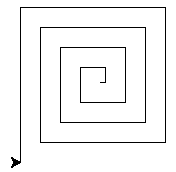
\includegraphics[scale=0.6]{images/boucle1.png}
\end{center}
\end{minipage}

\begin{exercice}{}

\begin{enumerate}
	\item Écrire une fonction \texttt{spirale1(n)} qui permet de tracer une spirale constituée de  \texttt{n}  carrés déformés.
	
\lignes{5}

	\item Écrire une fonction \texttt{spirale2(n, m)} qui permet de tracer une spirale constituée de  \texttt{n} polygones déformés à $m$ côtés.
	
\begin{minipage}{0.6\linewidth}
\medskip

	\lignes{7}
\end{minipage}\hfill
\begin{minipage}{0.35\linewidth}
	\begin{center}
	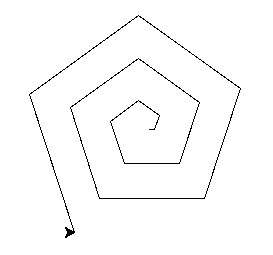
\includegraphics[scale=0.5]{images/spirale2.png}
	\end{center}
\end{minipage}

	
\end{enumerate}

\end{exercice}


\begin{entrainement}{}
 Écrire une fonction \texttt{spirale3(n, m)} qui permet de tracer une spirale constituée  de \texttt{n}   polygones réguliers concentriques  à $m$ côtés.
\begin{center}
	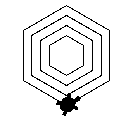
\includegraphics[scale=1]{images/spirale3.png}
	\end{center}

\end{entrainement}


\newpage

\section{Spécification et mise au point}

\subsection{Spécifier une fonction}

\begin{methode}{}

Si on écrit une bibliothèque de fonctions, il est nécessaire pour chaque fonction de décrire ce qu'elle fait à travers une documentation.

En Python, on peut associer à une fonction une \textbf{chaîne de documentation} ou \textit{docstring} où l'on spécifie :

\begin{itemize}
 \item les paramètres attendus par la fonction en précisant leur type ;
 \item des conditions sur les paramètres qu'on appelle \textbf{préconditions} ;
 \item le type de la valeur renvoyée (\texttt{None} s'il n'y a pas de \texttt{return}) ;
 \item ce qu'elle fait et/ou renvoie, on appelle cela une \textbf{postcondition}.
\end{itemize}



Par exemple, on peut spécifier ainsi une fonction calculant le PGCD de deux entiers naturels :

\begin{lstlisting}[style=rond]
def pgcd(a, b:):
	"""Paramètres : a et b deux entiers
	Préconditions : a >= 0 et b >= 0
	Valeur renvoyée : un entier
	Postcondition : renvoie le PGCD de a et b"""
	while b != 0:
		a, b = b, a % b
	return a  
\end{lstlisting}

En plaçant cette \textit{docstring} juste après la signature de la fonction, elle sera accessible à travers l'attibut \verb+__doc__+ ou la fonction \texttt{help} en mode interactif. 
Ce mécanisme d'introspection facilite l'appropriation d'une bibliothèque, un exemple avec la documentation de la fonction \texttt{randint} du module \texttt{random} : 

\begin{lstlisting}[style=compil]
>>> import random
>>> help(random.randint)
Help on method randint in module random:

randint(a, b) method of random.Random instance
    Return random integer in range [a, b], including both end points
>>> random.randint.__doc__
'Return random integer in range [a, b], including both end points.\n        '    
\end{lstlisting}

Depuis le mode interactif enrichi Ipython, on peut afficher plus de détails, avec le code source  :

\begin{lstlisting}[style=rond]    
In [2]: random.randint??
Signature: random.randint(a, b)
Docstring:
Return random integer in range [a, b], including both end points.
        
Source:   
    def randint(self, a, b):
        """Return random integer in range [a, b], including both end points.
        """

        return self.randrange(a, b+1)
File:      ~/anaconda3/lib/python3.8/random.py
Type:      method
\end{lstlisting}


À partir de  Python 3.5, on peut préciser de façon optionnelle le type attendu et le type renvoyé avec un mécanisme d'annotations. Ces \textbf{annotations de types} sont décrites dans  \url{https://mypy.readthedocs.io/en/stable/cheat_sheet_py3.html}.
\begin{lstlisting}[style=compil]
def greeting(name: str) -> str:
    return 'Hello ' + name
\end{lstlisting}

\end{methode}




\subsection{Mise au point de fonction et de programme}


\begin{methode}{}
Une \textbf{assertion} est une instruction qui vérifie si une  condition (à valeur booléenne) est  vérifiée dans l'état courant du programme.

L'exécution d'une  assertion est silencieuse si elle est vérifiée et elle lève une exception de type \texttt{AssertionError} qui interrompt l'exécution sinon.

La syntaxe est \texttt{assert condition}.


\begin{lstlisting}[style=compil]
>>> assert 1 == 1
>>> assert 1 == 2
Traceback (most recent call last):
  File "<stdin>", line 1, in <module>
AssertionError
\end{lstlisting}

On peut utiliser des assertions comme outils de \textbf{mise au point}  du programme   ou d'une fonction  en particulier. Considérons le cas de la fonction \texttt{ pgcd(a:int, b:int)->int} :


\begin{lstlisting}[style=rond]
def pgcd(a:int, b:int)->int:
	"""Paramètres : a et b deux entiers naturels
	Préconditions : a >= 0 et b >= 0
	Valeur renvoyée : un entier
	Postcondition : renvoie le PGCD de a et b"""
	#Vérification de précondition, programmation défensive
	assert isinstance(a,int) and isinstance(b,int) and a>=0   and b>=0
	while b != 0:
		a, b = b, a % b
	return a  
	
#tests unitaires, vérification de postconditions
assert pgcd(2,2) == 2                                                   
assert pgcd(2, 6) == 2                                                                                           
assert pgcd(45, 60) == 15                                              
assert pgcd(2, 0) == 2  
assert pgcd(0, 2) == 2 
\end{lstlisting}



\begin{itemize}
 \item On peut vérifier au début du corps de la fonction une \textbf{précondition} sur les paramètres, par exemple la précondition \textit{a entier positif} par \texttt{assert isinstance(a,int) and a>=0}. 
 
On parle de \textbf{programmation défensive}.
 
\item On peut définir en dehors de la fonction   \textbf{des tests unitaires} pour vérifier la \textbf{postcondition} sur quelques cas les plus couvrant possibles. On peut les rassembler dans une fonction ou un module externe pour constituer un  \textbf{jeu de tests}. 

\begin{lstlisting}[style=compil]
>>> def test_pgcd():  #jeu de test unitaires
...     assert pgcd(2,2) == 2
...     ............
...     assert pgcd(2, 0) == 2
...     print("Test unitaires réussis")
>>> test_pgcd()
"Test unitaires réussis"
\end{lstlisting}

Si le programme était incorrect, un test unitaire pourrait être faux et provoquer une erreur \texttt{Assertion Error}.



{\itshape \bfseries Cette méthodologie de mise au point de fonction peut être étendue à des programmes complets.}


\bcdanger{} Pour reprendre une citation célèbre d'\href{https://fr.wikipedia.org/wiki/Edsger_Dijkstra}{Edger Dijsktraa} :

\begin{quote}
{\itshape
Program testing can be used to show the presence of bugs, but never to show their absence! 
}
\end{quote}

\end{itemize}

\end{methode}

%\newpage

 \section{Portée d'une variable}
 
  \vspace*{-20pt}
 
 
 \begin{definition}{}
 
 \begin{itemize}
 
 \item Dans un code, la \textbf{portée d'une variable} définit les endroits du code où la variable est accessible.
 

 
 \item En \texttt{Python}, la portée d'une variable est lexicale \ie{} qu'elle est définie par l'endroit où la variable est définie.
 
 
  \item En  \texttt{Python}, une variable est \textbf{définie} dès qu'elle reçoit une valeur par une instruction d'\textbf{affectation}. 
  
  C'est la dernière instruction d'affectation associée à un nom de variable qui détermine la portée de cette variable.
  
  
\item  Il existe deux grandes catégories de variables en \texttt{Python} :
 
 \begin{itemize}
 	
 	\item Une variable définie dans une fonction est une \textbf{variable locale} à cette fonction, elle est accessible dans le bloc d'instruction de cette fonction et dans toutes les éventuelles fonctions qu'elle peut englober mais elle n'est pas visible dans tous les blocs qui englobent la fonction (programme principal ou fonctions englobantes).
 	\item  Une variable définie dans le programme principal (pas dans une fonction) est une \textbf{variable globale}, elle est accessible dans l'ensemble du code. 
 	
 \end{itemize}
 
 \item Un même nom de variable peut être utilisé dans une définition de variable par affectation à plusieurs niveaux d'imbrication de fonctions dans un même code.
 
 Pour déterminer la portée d'une variable utilisée à un endroit fixé du code, on applique la règle \textbf{LEGB} pour \textbf{Locale Englobante Globale Builtins}. On recherche d'abord la variable dans la portée de la fonction locale, puis dans la portée d'une fonction englobante, puis dans le programme principal à l'extérieur de toute fonction et enfin dans le module \texttt{builtins} qui est importé par défaut.
   
   
  \item Il est possible d'enfreindre la règle \textbf{LEGB} en utilisant le mot clef \textbf{global} si on veut définir une  variable dans une fonction avec une portée globale ou avec le  mot clef \textbf{nonlocal} si on veut définir  une  variable dans une fonction englobée avec une portée dans la fonction englobante.
 
 \item  La portée des variables en \texttt{Python} est très bien expliquée dans cette video : 
\begin{center}
\url{https://d381hmu4snvm3e.cloudfront.net/videos/qYPPwG7tu2eU/SD.mp4}
\end{center}

 \end{itemize}
 

 \end{definition}
 
 \vspace*{-20pt}
 
 
\begin{minipage}{0.45\linewidth}
\begin{programme}{}
 \begin{lstlisting}[style=rond]
a = 1

def f():
    a = 734
    print(a)
    
f()
print(a)
 \end{lstlisting}
\end{programme}
 \end{minipage}
 \hfill
 \begin{minipage}{0.45\linewidth}
\begin{programme}{}
 \begin{lstlisting}[style=rond]
a = 1

def f():
    a = a + 1
    print(a)
    
f()
print(a)
 \end{lstlisting}
\end{programme}
 \end{minipage}
 
 
 \begin{exercice}{}
 
 \begin{enumerate}
 	\item Que se passe-t-il lorsqu'on exécute les programmes 6 et 7 ci-dessus ? Commenter.
 	
 \lignes{6}
 
 
 
 \item Que se passe-t-il lorsqu'on exécute le programme 8 ci-dessous ? Commenter en précisant la portée des variables \texttt{a}, \texttt{b} et \texttt{c} lors de chaque exécution de l'instruction \texttt{print(a, b, c)}.
 	
 \lignes{6}
 
 
 \end{enumerate}
 \end{exercice}
 
 
 
 
\begin{programme}{}
\begin{lstlisting}[style=rond]
a, b, c = 731, 734, 735
def f():
    b, c = 736, 737
    def g():
        c = 738
        print(a, b, c)
    g()
    print(a, b, c)    
f()
print(a, b, c)
\end{lstlisting}
\end{programme}

\vspace*{-20pt}
 
\begin{exercice}{}
Que se passe-t-il lorsqu'on exécute le programme 9 ci-dessous ? Commenter en précisant la portée de la  variable \texttt{a} lors des appels successifs des fonctions \texttt{incremente1(a)}, \texttt{incremente2()} puis \texttt{incremente3()}.


 \lignes{10}
 
 
    
\end{exercice}


\begin{programme}{}
\begin{lstlisting}[style=rond]
def incremente1(a):
    a = a + 1
    
def incremente2():
    global a 
    a = a + 1
    
def incremente3():
    a = a + 1

a = 734
for k in range(10):
	incremente1(a)
print(a)
for k in range(10):
    incremente2()
print(a)
for k in range(10):
    incremente3()
print(a)
\end{lstlisting}
\end{programme}




%\newpage


\tableofcontents

\end{document} %  ======================  FIN  ==========================